% Format teze zasnovan je na paketu memoir
% http://tug.ctan.org/macros/latex/contrib/memoir/memman.pdf ili
% http://texdoc.net/texmf-dist/doc/latex/memoir/memman.pdf
% 
% Prilikom zadavanja klase memoir, navedenim opcijama se podešava 
% veličina slova (12pt) i jednostrano štampanje (oneside).
% Ove parametre možete menjati samo ako pravite nezvanične verzije
% mastera za privatnu upotrebu (na primer, u b5 varijanti ima smisla 
% smanjiti 
\documentclass[12pt,oneside]{memoir}

% Paket koji definiše sve specifičnosti mastera Matematičkog fakulteta
\usepackage[latinica]{matfmaster}
\usepackage{graphicx}

% Paket koji obezbeđuje ispravni prikaz ćiriličkih italik slova kada
% se koristi pdflatex. Zakomentarisati ako na sistemu koji koristite ovaj
% paket nije dostupan ili ako ne radi ispravno.
\usepackage{cmsrb}
\usepackage[font={small}]{caption}
% Ostali paketi koji se koriste u dokumentu
\usepackage{listings} % listing programskog koda
\usepackage{color} %use color
\usepackage{enumitem}
\usepackage{xurl}

% Podrazumevano pismo je ćirilica.
%   Ako koristite pdflatex, a ne xetex, sav latinički tekst na srpskom jeziku
%   treba biti okružen sa \lat{...} ili \begin{latinica}...\end{latinica}.
%
% Opicija [latinica]:
%   ako želite da pišete latiniciom, dodajte opciju "latinica" tj.
%   prethodni paket uključite pomoću: \usepackage[latinica]{matfmaster}.
%   Ako koristite pdflatex, a ne xetex, sav ćirilički tekst treba biti
%   okružen sa \cir{...} ili \begin{cirilica}...\end{cirilica}.
%
% Opcija [biblatex]:
%   ako želite da koristite reference na više jezika i umesto paketa
%   bibtex da koristite BibLaTeX/Biber, dodajte opciju "biblatex" tj.
%   prethodni paket uključite pomoću: \usepackage[biblatex]{matfmaster}
%
% Opcija [b5paper]:
%   ako želite da napravite verziju teze u manjem (b5) formatu, navedite
%   opciju "b5paper", tj. prethodni paket uključite pomoću: 
%   \usepackage[b5paper]{matfmaster}. Tada ima smisla razmisliti o promeni
%   veličine slova (izmenom opcije 12pt na 11pt u \documentclass{memoir}).
%
% Naravno, opcije je moguće kombinovati.
% Npr. \usepackage[b5paper,biblatex]{matfmaster}

% Pomoćni paket koji generiše nasumičan tekst u kojem se javljaju sva slova
% azbuke (nema potrebe koristiti ovo u pravim disertacijama)

\definecolor{mygreen}{rgb}{0,0.6,0}
\definecolor{mygray}{rgb}{0.5,0.5,0.5}
\definecolor{mymauve}{rgb}{0.58,0,0.82}
\definecolor{lightgray}{rgb}{.9,.9,.9}
\definecolor{darkgray}{rgb}{.4,.4,.4}
\definecolor{purple}{rgb}{0.65, 0.12, 0.82}
\definecolor{codegray}{gray}{0.9}
\newcommand{\code}[1]{\allowbreak{\colorbox{codegray}{\texttt{\scalebox{0.9}{#1}}}}}%

\newcounter{shellRef}[chapter]

\newcommand{\shellcmd}[2]{\\\\\texttt{\footnotesize\$ #1 \null\hfill (\refstepcounter{shellRef}{\theshellRef})\label{#2} }\\\\}
\renewcommand{\theshellRef}{\thechapter.\number\numexpr\value{shellRef}\relax}

\let\origthelstnumber\thelstnumber
\makeatletter
\newcommand*\Suppressnumber{%
  \lst@AddToHook{OnNewLine}{%
    \let\thelstnumber\relax%
     \advance\c@lstnumber-\@ne\relax%
    }%
}

\newcommand*\Reactivatenumber[1]{%
  \setcounter{lstnumber}{\numexpr#1-1\relax}
  \lst@AddToHook{OnNewLine}{%
   \let\thelstnumber\origthelstnumber%
   \refstepcounter{lstnumber}
  }%
}

\setcounter{tocdepth}{3}
\setcounter{secnumdepth}{3}
\setsecnumdepth{subsection}
% \renewcommand\thesubsection{(\alph{subsection})}

\hyphenation{Functional-Element HTML-Functional-Element}
\makeatother
% %Customize a bit the look
% \lstset{ %
% backgroundcolor=\color{white}, % choose the background color; you must add \usepackage{color} or \usepackage{xcolor}
% basicstyle=\footnotesize, % the size of the fonts that are used for the code
% breakatwhitespace=false, % sets if automatic breaks should only happen at whitespace
% breaklines=true, % sets automatic line breaking
% captionpos=b, % sets the caption-position to bottom
% commentstyle=\color{mygreen}, % comment style
% deletekeywords={...}, % if you want to delete keywords from the given language
% escapeinside={\%*}{*)}, % if you want to add LaTeX within your code
% extendedchars=true, % lets you use non-ASCII characters; for 8-bits encodings only, does not work with UTF-8
% frame=false, % adds a frame around the code
% keepspaces=true, % keeps spaces in text, useful for keeping indentation of code (possibly needs columns=flexible)
% keywordstyle=\color{blue}, % keyword style
% % language=Octave, % the language of the code
% morekeywords={*,...}, % if you want to add more keywords to the set
% numbers=left, % where to put the line-numbers; possible values are (none, left, right)
% numbersep=5pt, % how far the line-numbers are from the code
% numberstyle=\tiny\color{mygray}, % the style that is used for the line-numbers
% rulecolor=\color{black}, % if not set, the frame-color may be changed on line-breaks within not-black text (e.g. comments (green here))
% showspaces=false, % show spaces everywhere adding particular underscores; it overrides 'showstringspaces'
% showstringspaces=false, % underline spaces within strings only
% showtabs=false, % show tabs within strings adding particular underscores
% stepnumber=1, % the step between two line-numbers. If it's 1, each line will be numbered
% stringstyle=\color{mymauve}, % string literal style
% tabsize=2, % sets default tabsize to 2 spaces
% title=\lstname % show the filename of files included with \lstinputlisting; also try caption instead of title
% }
%END of listing package%
 

%define Javascript language
\lstdefinelanguage{JavaScript}{
keywords={typeof, const, class, interface, this, get, string, number, extends, export, new, true, false, catch, function, return, null, catch, let, switch, var, if, in, while, do, else, case, break},
keywordstyle=\color{blue}\bfseries,
ndkeywords={export, boolean, throw, implements, extends, public, abstract, protected, import, from, private},
ndkeywordstyle=\color{red}\bfseries,
identifierstyle=\color{black},
sensitive=false,
comment=[l]{//},
morecomment=[s]{/*}{*/},
commentstyle=\color{purple}\ttfamily,
stringstyle=\color{mygreen}\ttfamily,
moredelim=[s][\color{black}]{\$\{}{\}}, % same as morestring in this case
morestring=[d]{'},
morestring=[d]{`},
morestring=[d]{"},
}

\lstdefinelanguage{html}{
keywords={body, div, div,span, i, script, h1, const},
keywordstyle=\color{blue}\bfseries,
ndkeywords={class, export, boolean, throw, implements, import, this},
ndkeywordstyle=\color{darkgray}\bfseries,
identifierstyle=\color{black},
sensitive=false,
comment=[l]{//},
morecomment=[s]{/*}{*/},
commentstyle=\color{purple}\ttfamily,
stringstyle=\color{mygreen}\ttfamily,
morestring=[b]',
morestring=[b]"
}


\lstdefinelanguage{shell}{
keywords={\$, \> },
keywordstyle=\color{red}\bfseries,
ndkeywords={class, export, boolean, throw, implements, import, this},
ndkeywordstyle=\color{darkgray}\bfseries,
identifierstyle=\color{black},
sensitive=false,
morecomment=[s]{/*}{*/},
commentstyle=\color{purple}\ttfamily,
stringstyle=\color{mygreen}\ttfamily,
morestring=[b]',
morestring=[b]`,
morestring=[b]"
}


\lstset{
language=JavaScript,
extendedchars=true,
basicstyle=\footnotesize\ttfamily,
backgroundcolor=\color{white},
showstringspaces=false,
showspaces=false,
numbers=none,
numberstyle=\footnotesize,
escapeinside=||,
numbersep=9pt,
tabsize=2,
breaklines=true,
showtabs=false,
captionpos=b,
}

\lstset{
language=shell,
extendedchars=true,
basicstyle=\footnotesize\ttfamily,
backgroundcolor=\color{lightgray},
frame=single,
showstringspaces=false,
showspaces=false,
numbers=none,
numberstyle=\footnotesize,
numbersep=9pt,
tabsize=2,
breaklines=true,
showtabs=false,
captionpos=b
}

\lstdefinestyle{htmlStyle} {language=html,backgroundcolor=\color{white},frame=single}
\lstdefinestyle{jsStyle} {language=JavaScript, escapeinside=||, backgroundcolor=\color{white},frame=single, numbers=left, numberstyle=\tiny, }
\lstdefinestyle{shellStyle} {language=shell,backgroundcolor=\color{lightgray},frame=single}

\renewcommand\lstlistingname{Primer koda}
\setlist[enumerate]{itemsep=0mm}
% Datoteka sa literaturom u BibTex tj. BibLaTeX/Biber formatu
\bib{AleksandarMilosavljevic_master-rad}

% Ime kandidata na srpskom jeziku (u odabranom pismu)
\autor{Aleksandar Milosavljević}
% Naslov teze na srpskom jeziku (u odabranom pismu)
\naslov{Razvoj okruženja "Pure" za razvoj veb interfejsa}
% Godina u kojoj je teza predana komisiji
\godina{2021}
% Ime i afilijacija mentora (u odabranom pismu)
\mentor{dr Saša \textsc{Malkov}, vanredni profesor\\ Univerzitet u Beogradu, Matematički fakultet}
% Ime i afilijacija prvog člana komisije (u odabranom pismu)
\komisijaA{dr Aleksandar \textsc{Kartelj}, docent\\ Univerzitet u Beogradu, Matematički fakultet}
% Ime i afilijacija drugog člana komisije (u odabranom pismu)
\komisijaB{dr Ivan \textsc{Čukić}, docent\\ Univerzitet u Beogradu, Matematički fakultet}
% Ime i afilijacija trećeg člana komisije (opciono)
% \komisijaC{}
% Ime i afilijacija četvrtog člana komisije (opciono)
% \komisijaD{}
% Datum odbrane (obrisati ili iskomentarisati narednu liniju ako datum odbrane nije poznat)
\datumodbrane{27. septembar 2021.}

% Apstrakt na srpskom jeziku (u odabranom pismu)
\apstr{%
U okviru ovog rada predstavljen je razvoj okruženja \emph{Pure} - modernog okruženja za razvoj veb aplikacija baziranog na obrascu \emph{Flux}. U narednim poglavljima nalaze se obrazloženja za odabir konkretnih alata i biblioteka tokom implementacije, primeri korišćenja okruženja za pisanje korisničkih aplikacija kao i objašenje implementacionih detalja najvažnijih elemenata okruženja.
}

% Ključne reči na srpskom jeziku (u odabranom pismu)
\kljucnereci{veb, internet, interfejs, HTML, CSS, JavaScript, TypeScript, razvojno okruženje, React, Angular, Redux, Flux, MVC}

\begin{document}
% ==============================================================================
% Uvodni deo teze
\frontmatter
% ==============================================================================
% Naslovna strana
\naslovna
% Strana sa podacima o mentoru i članovima komisije
\komisija
% Strana sa posvetom (u odabranom pismu)
\posveta{
  Mojim roditeljima.
}
% Strana sa podacima o disertaciji na srpskom jeziku
\apstrakt
% Sadržaj teze
\tableofcontents*

% ==============================================================================
% Glavni deo teze
\mainmatter
% ==============================================================================

% ------------------------------------------------------------------------------
\chapter{Uvod}
Iako današnji mini računari, koje gotovo svi nosimo u džepu, imaju više procesorske snage 
nego računar koji je korišćen tokom Appolo misije \cite{apollo}, 
danas te lične računare ne koristimo za teška izračunavanja i komplikovane procedure. 
Koristimo ih najčešće kao jednostavne terminale kako bismo pristupili internet resursima,
to jest, podacima koji se nalaze na velikim centralizovanim računarskim sistemima. 
Veb interfejs je tako postao glavni način naše interakcije sa računarom i internetom.

Posledica toga je značajna promena fokusa u svetu razvoja aplikativnog softvera.
Ukoliko pogledamo rezultat upitnika kompanije \emph{"Stack Overflow"}
o najkorišćenijim programerskim alatima, videćemo da prva dva mesta na listi
zauzimaju upravo veb tehnologije (Na prvom mestu je JavaScript sa 69.7\%, dok je na 
drugom HTML/CSS sa 62.4\%) \cite{StackOverflowSurvey}.

Kako potreba za novim softverom daleko prevazilazi mogućnost softverskih inženjera 
da taj softver isporuče, biblioteke i okruženja koja pomažu pri razvoju softvera 
postali su veoma važan deo skupa inženjerskih alata.
U domenu razvoja veb aplikacija, na tržištu se izdvajaju tri razvojna okruženja. 
Ova tri razvojna okruženja najviše se međusobno razlikuju po pristupu u promeni 
stanja aplikacije i razumevanju
toga šta je centralni deo dizajna (u funkcionalnom smislu) jedne veb aplikacije.

Kada posmatramo ova popularna razvojna okruženja, uočavamo dva bitno različita 
pristupa u arhitekturi:
\begin{enumerate}
  \item Obrazac \emph{Model-Pogled-Upravljač} u kom aplikacija predstavlja skup
   povezanih komponenti organizovanih u hijerarhisku strukturu, kojima je 
   pridruženo stanje i ponašanje.
  \item Obrazac \emph{Flux} u kom se aplikacija posmatra kao mašina stanja čija je 
  vizuelna reprezentacija samo rezultat trenutnog stanja.
\end{enumerate}

Prvi pristup je prisutan u okruženju \emph{Angular}, drugi je dominantan u biblioteci 
\emph{React}, dok okruženje \emph{Vue.js} zastupa dizajn koji predstavlja kompromis izmеđu ova dva pristupa.

Ovaj rad se bavi projektovanjem i razvojem okruženja \emph{Pure}, koje predstavlja
savremeno razvojno okruženje za pisanje veb interfejsa po arhitekturi SPA, a koje 
predstavlja pokušaj objedinjavanja najboljih elemenata obrazaca \emph{Model-Pogled-Upravljač} i \emph{Flux}.
\section{Organizacija rada}
U poglavlju \ref{chap:SPA} opisaćemo arhitekturu SPA, kao najčešći arhitekturalni obrazac korišćen pri
izradi veb aplikacija; osvrnuti na najčešće probleme pri implementiranju ovog arhitekturalnog obrasca kroz analizu
najpopularnijih razvojnih okruženja i objasniti motivaciju
za pisanje novog razvojnog okruženja. U poglavlju \ref{chap:koncept} definisaćemo formalne zahteve koje bi novo okruženje
trebalo da ispuni.
Nakon toga, u poglavlju \ref{chap:pure-okruzenje}, upoznaćemo se sa novorazvijenim okruženjem za razvoj SPA aplikacija iz perspektive korisnika (inženjera).
U poglavlju \ref{chap:pure-implementacija} ćemo se upoznati sa implementacionim detaljima samog orkuženja.
U poglavlju \ref{chap:diskusija} daćemo objašenje na koji način su ispunjeni zahtevi postavljeni u poglavlju \ref{chap:koncept}
i analizirati novorazvijeno rešenje iz perspektive budućih proširenja i unapređenja.






% ------------------------------------------------------------------------------
\chapter{Arhitektura SPA}\label{chap:SPA}
Poboljšanjem infrastrukture Interneta i napredovanjem tehnologije i mogućnosti
ličnih računara
i mobilnih uređaja, prezentaciona logika korisničkih aplikacija se postepeno
selila sa centralizovanih
serverskih računara na klijentske uređaje. Arhitektura SPA (eng. \emph{Single Page Application}) je dovela ovaj princip
do krajnjih granica
prebacivanjem celokupne logike ponašanja aplikacije na klijentsku stranu \cite{SPA}.
Iako SPA nije sama po sebi arhitektura, već samo akronim koji služi za opis osnove 
funkcionisanja klijentske aplikacije,
ovaj opis implicitno definiše obrazac komunikacije između servera i klijenta,
pa posredno utiče i na sam arhitekturalni obrazac celopkupne aplikacije. U ovom arhitekturalnom obrascu klijent
pri prvom zahtevu
ka serveru u osnovi preuzima celokupni (klijentski) aplikativni k\^od i obrađuje ga u
pregledaču, dok
svi naredni pozivi služe prostoj razmeni podataka. Ovo je značajno uticalo
na samu metodologiju razvoja veb aplikacija.
\begin{figure}[!ht]
  \centering
  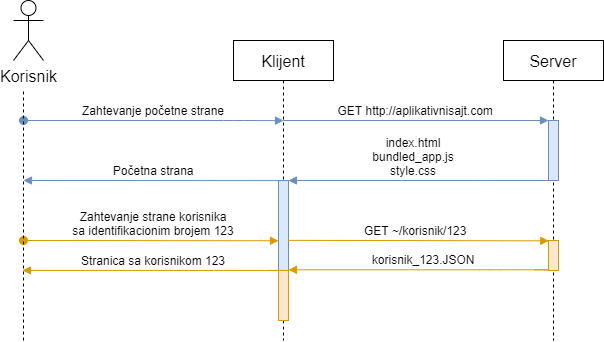
\includegraphics[width=0.8\textwidth]{slike/SPA_Diagram.drawio.png}
  \caption{Dijagram sekvence komunikacije u SPA aplikaciji.}
  \label{fig:SPA}
\end{figure}\\
Ovaj pristup omogućio je razdvajanje poslova timova zaduženih za
serversku logiku i timova zaduženih za prezentacionu logiku i vizuelni dizajn,
a time omogućio i veći stepen njihove nezavisnosti.
Jedina tačka spajanja ova dva tima postao je dizajn interfejsa
između klijentske i serverske aplikacije. Rešenje ovog problema inženjeri su našli
u definisanju skupa arhitekturalnih smernica koji su nazvali REST (eng. \emph{Representational State Transfer}) \cite{REST}.

REST je standardizovao način organizacije podataka
i način pristupanju podacima kroz API (eng. \emph{Application Programmable Interface}). 
REST daje smernice u okviru organizacije podataka (resursa). Po REST-u podaci bi trebalo da budu organizivani po hijerarhijskom modelu
strukture fajl-sistema.
\pagebreak

\noindent
Odvajanjem razvoja klijentskih i serverskih aplikacija, pisanje složenih korisničkih aplikacija postalo je značajno lakše.
Povećavanjem složenosti razvoja ovih aplikacija,
razvila se potreba za razvojnim obrascima i razvojnim okruženjima koja omogućavaju
programerima da lakše organizuju svoj k\^od i da lakše njime upravljaju.
Prvi obrazaci koji su se koristili preuzeti su iz arhitekture višestraničnih aplikacija.
Primer jednog takvog obrasca je \emph{Model-Pogled-Upravljač} (eng. \emph{Model-View-Controller}) \cite{MVC}. 

\section{Obrazac Model-Pogled-Upravljač}

Obrazac \emph{Model-Pogled-Upravljač} nastao je pre pojave SPA.
Koristio se za velike sajtove i aplikacije, ali na takav način da su sve komponente pisane
kao serverski k\^od. Ideja obrasca \emph{Model-Pogled-Upravljač} je da omogući razdvajanje odgovornosti
između logike podataka, aplikativne logike i vizuelne reprezentacije programa.
\begin{figure}[!ht]
  \centering
  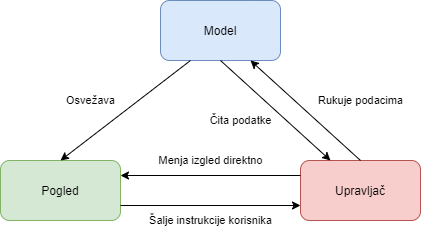
\includegraphics[width=0.7\textwidth]{slike/MVC_pattern.drawio.png}
  \caption{Arhitektura obrasca Model-Pogled-Upravljač}
  \label{fig:MVC}
\end{figure}
\\
\\
Ovaj obrazac ima sličnu primenu i u SPA aplikacijama, sa tom razlikom što se sve odvija na klijentu.
Umesto apstrakcije nad bazom podataka, \emph{model} predstavlja apstrakciju nad podacima učitanim
u aplikaciju. \emph{Upravljač} (ili kontroler) je zadužen za aplikativnu logiku i za prihvatanje
instrukcija poslatih sa nivoa \emph{pogleda}. Sloj \emph{pogleda} služi za opis vizuelne
reprezentacije aplikacije i ne sadrži nikakvu aplikativnu logiku. Najpoznatiji predstavnik okruženja
koja koriste ovaj obrazac je \emph{Angular} \cite{Angular}.

\section{Obrazac Flux}
Obrazac \emph{Flux} je nastao u kompaniji \emph{Facebook}, iz potrebe inženjera da otklone probleme sa 
deljenjem stanja između različitih komponenti i čestim nadmetanjem za resurse (eng. \emph{race condition}) \cite{raceCondition}.
Baziran je na ustaljenim arhitekturama funckionalnog i reaktivnog programiranja.
\begin{figure}[!ht]
  \centering
  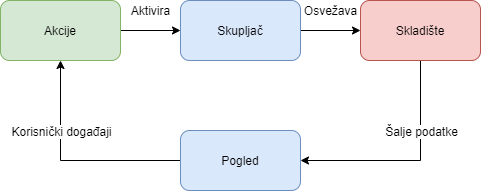
\includegraphics[width=0.7\textwidth]{slike/FLUX_pattern.png}
  \caption{Arhitektura obrasca Flux}
  \label{fig:flux}
\end{figure}
\\
Osnovna ideja ovog obrasca je da podaci teku u jednom smeru, tako da se uvek može jednostavno
utvrditi redosled akcija i na taj način sprečiti nadmetanje za resurse između različitih komponenti.
U оbrscu \emph{Flux} se izmene stanja u modelu izvršavaju
atomično\footnote{Atomično - Nedeljiva celina. Atomična operacija se izvršava po principu "sve ili ništa".}
na glavnoj niti, pa nema nadmetanja za resursima.

\emph{Pogled}, kao i kod obrasca \emph{Model-Pogled-Upravljač}, služi za opis vizualne reprezentacije programa.
\emph{Pogled} utiče na tok podataka tako što pri korisničkom događaju odabire \emph{akciju} koju će da emituje
ka \emph{skupljaču} (eng. \emph{reducer}).

\emph{Skupljač} je čista funkcija \cite{functionalProgramming}, koja kao argumente
prihvata akciju i trenutno stanje skladišta i vraća novo stanje skladišta.
Povratna vrednost skupljača se potom upisuje u skladište umesto starog stanja, tako da ne postoji slučaj deljenja iste reference objekta
između dve komponenente. Sloj pogleda jedne komponente može samo da pročita stanje skladišta, ali ne i da ga menja neposredno, već na njega može da utiče
isključivo okidanjem neke akcije. Nakon obrade akcije, skladište okruženja sadrži novi objekat i tako zna da mora da osveži iscrtavanje DOM-a \cite{DOM}.

DOM (eng. \emph{Document Object Model}) je memorijska reprezentacija HTML dokumenta organizovana tako
da bude pogodna za upravljanje iz koda napisanog u jeziku \emph{JavaScript}. 
\begin{figure}[!ht]
  \centering
  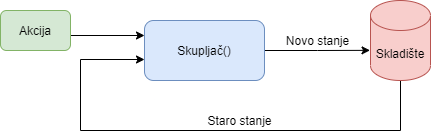
\includegraphics[width=0.7\textwidth]{slike/Reducer.png}
  \caption{Skupljač}
  \label{fig:reducer}
\end{figure}
\\
Važno je naglasiti da obrazac \emph{Flux} za razliku od obrasca \emph{Model-Pogled-Upravljač} ne insistira
na podeli slojeva po fajl strukturi na takav način da dva sloja ne mogu biti deo istog fajla.
Razdvajanje odgovornosti se ovde posmatra u domenu toka podataka i toga koji sloj može
upravljati i pristupati podacima u \emph{kom trenutku}. Biblioteka \emph{React} nastala je u kompaniji \emph{Facebook} kao predstavnik ovog obrasca \cite{React}.
% ------------------------------------------------------------------------------
% ------------------------------------------------------------------------------

\section{Problemi sa okruženjem Angular}\label{problemi:ang}
Okruženje \emph{Angular} popularno je među programerima koji razvijaju softver za korporativne korisnike.
Razvojni timovi koji rade na razvoju ovakvog softvera često broje preko 20 inženjera i testera.
Obrazac \emph{Model-Pogled-Upravljač} koji prestavlja osnovni arhitekturalni dizajn okruženja Angular,
značajno olakšava rad velikom broju ljudi na istom programskom kodu.
\subsection{Upravljanje stanjem} \label{subsec:upravljanje-stanjem}

Problem sa okruženjem \emph{Angular} nastaje kada među različitim komponentama moramo da delimo stanje.
Nadmetanje za resursima vremenom počinje da se javlja sve češće kao problem, a "pametna krpljenja" počinju
da zauzimaju sve veći deo programskog koda.

Problem sa deljenjem stanja, pored problema sa nadmetanjem za resurse, je i taj što aplikacija postaje previše kompleksna
za razumevanje čak i za iskusnije inženjere i problemi u kodu se vremenom sve bolje sakrivaju,
čekajući na krajnje korisnike.


\subsection{Logika u pogledu} \label{subsec:logika-u-pogledu}
Pogledajmo jedan primer koda sa sajta \url{https://angular.io/}:
\begin{lstlisting}[style=htmlStyle, caption={Primer koda u \emph{Angular}-u},label=angular:code]
<div *ngFor="let item of items">{{item.name}}</div>
\end{lstlisting}
K\^od prikazan u primeru \ref{angular:code} predstavlja instrukciju za izlistavanje stavki (\code{item}) iz niza \code{items}.
Drugim rečima, ovo nije HTML\footnote{Hyper-Text-Markup-Language.}-element, već instrukcija napisana na 
specijalnom jeziku okruženja \emph{Angular}, namenjenom za opisivanje
pogleda, koja će u vreme izvršavanja biti zamenjena pravim HTML-elementom. Ovaj HTML-element će dinamički promeniti svoj sadržaj
svaki put kada se sadržaj niza \code{items} promeni. 

Ovo je jednostavan primer, ali nije teško zamisliti situaciju u kojoj programska logika postaje previše kompleksna
da bi se o njoj rezonovalo u slučaju potrage za greškom. Da stvar bude gora, ovu logiku nije moguće (jednostavno) debagovati\footnote{\emph{Debug} - eng. Traženje i uklanjanje grešaka.}
modernim alatima ugrađenim u pregledače,
jer logika ispisana u ovoj instukciji prolazi kroz više faza prevođenja i uglavnom je na kraju izvršava
optimizovani i minifikovani k\^od samog okruženja, koji je veoma nečitljiv.
\section{Problemi sa bibliotekom React}\label{problemi:react}
Okruženje \emph{React} razvijeno je od strane \emph{Facebook} inženjera sa ciljem da stvore okruženje
dizajnirano tako da obrazac \emph{Flux} bude lak za implementaciju pri razvoju aplikacija.
Ovaj arhitekturalni obrazac okruženja omogućio je u velikoj meri izbegavanje problema nadmetanja za resurse, ali
su neki drugi problemi ipak ostali deo rešenja.
\subsection{Razdvajanje odgovornosti} \label{subsec:razdvajanje-odgovornosti}
U primerima \ref{file:react.jsx} i \ref{file:react.js} vidimo primer preuzet sa zvanične veb stranice biblioteke \emph{React}.
U pitanju su dva različita načina definisanja komponente u okruženju \emph{React}. U primeru \ref{file:react.jsx}
je prikazan način koji koristi sintaksu \emph{JSX}. \emph{JSX} je skraćenica za \emph{JavaScript-XML}, što može da se uoči i iz prikazanog primera.
Ideja je da se komponenta može u potpunosti opisati u jednom fajlu sa ekstenzijom \code{.jsx} (ili \code{.tsx} ako koristite \emph{TypeScript} \cite{TypeScript}).

Umesto posebnog fajla koji bi koristio HTML-sintaksu (ili sintaksu nalik HTML-sintaksi, kao što je to slučaj u okruženju \emph{Angular}),
u biblioteci \emph{React}, struktura komponente može se opisati na istom mestu gde i ponašanje komponente.
Ovo često omogućava lakše rezonovanje o povezanosti vizualne strukture komponente i njenog ponašanja i predstavlja
pristup razdvajanja odgovornosti na nivou komponenenata, a ne na nivou tehnologije. 

Ovaj mehanizam se u u pozadini ostvaruje tako što React transpiluje\footnote{Transpilacija - prevođenje sa jednog jezika na drugi, viši programski jezik.}
ovaj k\^od na čist \emph{JavaScript} (Primer \ref{file:react.js}).
Korisnik može svoje komponente pisati i na način prikazan u primeru \ref{file:react.js}, ali je
primer \ref{file:react.jsx} očigledno lakši za čitanje i rezumevanje strukture.
\\
\\
\noindent\begin{minipage}[b]{.46\textwidth}
\begin{lstlisting}[style=htmlStyle, numbers=left, numberstyle=\tiny, caption={JSX-sintaksa},label=file:react.jsx]
const element = (
  <h1 className="greeting">
    Hello, world!
  </h1>
);
\end{lstlisting}
\end{minipage}
\hfill
\begin{minipage}[b]{.46\textwidth}
\begin{lstlisting}[style=jsStyle, caption={HTML-sintaksa},label=file:react.js]
const element = React.createElement(
  'h1',
  {className: 'greeting'},
  'Hello, world!'
);
\end{lstlisting}
\end{minipage}
\\
Iako je ovo veoma zgodan mehanizam, on uvodi neke neželjene posledice. Naime, jako je teško utvrditi šta je ispravan,
a šta neispravan \emph{JSX} k\^od i gde su tačno granice gde počinje HTML, a zavšava se \emph{JavaScript}. To možemo uočiti i na
primeru \ref{file:react.jsx}. Element \code{<h1>} u ovom primeru ima postavljenu vrednost atributa \code{className} na nisku \code{''greeting''}.
Ovaj atribut zapravo se pri prevođenju na HTML, tumači kao \code{class}. Razlog zašto ne koristimo reč \code{class}
u \emph{JSX} kodu je taj što je \code{class} rezervisana reč u \emph{JavaScript}-u.

Ovo je samo jedan dobro poznat primer koji zbunjuje nove korisnike, ali sličnih, a bolje sakrivenih primera ima dosta.
Ovaj sistem opisa vizuelne strukture podleže gotovo istim problemima kao i \emph{Angular}-ov jezik za opis strukture (eng. \emph{Templating language}),
jer nad njim ne možemo koristi napredne alate za debagovanje.
\\
\\

\subsection{Okruženje ili biblioteka}
Iako \emph{React} nije razvojno okruženje u punom smislu te reči, već biblioteka koja se bavi isključivo opisom sloja pogleda,
mnogi inženjeri ga koriste u sklopu ekosistema kao deo razvojnog okruženja.
Sve ostale funkcionalnosti koje su neophodne za kompletno razvojno okruženje deo su drugih biblioteka (\emph{ReactDOM, Redux, MobX, ...}).
Ovo dovodi do velike heterogenosti u pristupu pisanja koda i zbog toga nema jedinstvenog pristupa rešavanju većini problema
koji se javljaju pri razvoju aplikacija. Ovo je upravo razlog zbog kojeg je \emph{Angular} u velikim korporacijskim okruženjima i timovima
i dalje dominantan izbor.

\section{Motivacija za pravljenje novog okruženja}
Motivacija pri pravljenju novog okruženja potiče iz želje za ispitivanjem
alternativnog pristupa pravljenju jedinstvenog okruženja. Novo okruženje bi trebalo
da počiva na temeljima dobrih aspekata postojećih rešenja, kombinujući ih tamo
gde to ima smisla. U delovima dizajna u kojima nijedno od postojećih okruženja
nema adekvatan odgovor na predstavljene probleme, novo okruženje bi trebalo
da ponudi novo i originalno rešenje problema.

Ukratko, novo okruženje treba da bude moderan alat za razvoj klijentskih
veb aplikacija koje u svom dizajnu ne sadrži opisane greške iz predstavljenih rešenja.

% ------------------------------------------------------------------------------
\chapter{Koncept okruženja Pure}\label{chap:koncept}
U ovom poglavlju ćemo definisati formalne zahteve i objasniti osnovne koncepte na kojima treba da počiva
okruženje \emph{Pure}.

\section{Zahtevi}\label{sec:zahtevi}
Kako bismo imali jasnu ideju kako bi novo okruženje, koje rešava opisane probleme,
trebalo da izgleda, ovde ćemo definisati formalne zahteve koje bi novo
okruženje trebalo da ispuni.  
\begin{enumerate}
  \item Kako bismo izbegli probleme iz predstavljenih okruženja kao što su
  \emph{logika u pogledu} (Odeljak \ref{subsec:logika-u-pogledu}) i
  \emph{razdvajanje odgovornosti} (Odeljak \ref{subsec:razdvajanje-odgovornosti})
  novo okruženje ne sme da uvodi novi, niti da koristi bilo kakav postojeći
  specijalizovani jezik za opisivanje strukture HTML-a. Dodatni zahtev u pogledu
  opisa HTML-strukture komponenenata je omogućavanje debagovanja
  logike i strukture izgleda komponente alatima koji su ugrađeni u moderne pregledače. \label{zahtev:1}
  \item 
  Kako bi se izbegao problem sa deljenjem stanja (Odeljak \ref{subsec:upravljanje-stanjem}),
  novo okruženje bi trebalo da
  se oslanja na obrazac \emph{Flux} i jednosmeran tok podataka.
  Stanje mora biti centralizovano, a interfejs za upravljanje stanjem
  mora biti robustan i univerzalan za sve komponente.
  \label{zahtev:2}
 \item Kako bi što manje grešaka došlo do korisnika, potrebno je uočiti
 što više grešaka koje je moguće uočiti u fazi razvoja kroz podršku striktnih tipova.
 \label{zahtev:3}
 \item Distribucija razvojnog okruženja mora biti dostupna kroz
 javni repozitorijum \emph{npm}-paketa. \label{zahtev:4}
 \item Okruženje mora biti otvoreno za modifikovanje, kako u smislu prilagođavanja okruženja konkretnom projektu,
tako i u smislu predloga za modifikovanje samog okruženja kroz \emph{zajednicu otvorenog koda} (eng. \emph{Open Source community}.). \label{zahtev:5}
 \item Komponente okruženja moraju imati jednostavnu i lako čitljivu strukturu. \label{zahtev:6}
\end{enumerate}

\section{Arhitektura i dizajn okruženja}
Novo okruženje preuzeće obrazac \emph{Flux} od biblioteke \emph{React}, ali smernice za konretnu implementaciju ovog obrasca
biće preuzete od biblioteke \emph{NgRx} koja je deo \emph{Angular}-ekosistema \cite{NgRx}. Od okruženja \emph{Angular}
takođe će biti preuzet pristup razvoju koji podrazumeva pisanje komponenti u jeziku \emph{TypeScript} umesto jezika \emph{JavaScript}.
\subsection{Zašto ne HTML?} \label{subsec:zasto-ne-html}
Iako je HTML oproban jezik za opisivanje strukture dokumenta, on ima svoja ograničenja koja nije tako lako prevazići.
Tekst editori pri pisanju HTML fajla uglavnom teško mogu da zaključe kontekst povezivanja
pojedinačnih HTML-elemenata sa konkretnim funkcijama i promenljivim napisanim u \emph{JavaScript}-u i zbog toga je podrška alata,
a samim tim i iskustvo tokom pisanja HTML koda, značajno slabije nego pri pisanju \emph{JavaScript} ili \emph{TypeScript} koda.
Dodatna mana je u tome što je jako teško segmentirati HMTL k\^od u hijerarhijsku strukturu ili ga podeliti na više fajlova,
jer u HTML-u ne postoji opcija za uključivanje potkomponenti.
Korišćenjem \emph{TypeScript} funkcija umesto sintakse HTML-a rešavaju se ovi problemi.
Alati za upravljanje \emph{TypeScript} kodom značajno su napredniji od alata za upravljanje HTML-om.

\section{Ime okruženja}
Ime okruženja \emph{Pure}\footnote{\emph{Pure} - eng. Čisto, čist.} inspirisano je 
funkcionalnom paradigmom i čistim funkcijama \cite{functionalProgramming}. Funkcionalni elementi (koji će biti opisani u ovom poglavlju),
predstavljaju uslovno rečeno čiste funkcije, koje prihvataju trenutno stanje kao argument i vraćaju
DOM-element kao rezultat. Ovo nam omogućava da implementiramo i mehanizam memoizacije (eng. \emph{Memoization}) \cite{functionalProgramming},
koji je iskorišćen kao mehanizam optimizacije.

Drugi razlog za ime \emph{Pure} dolazi iz činjenice da okruženje koristi isključivo \emph{JavaScript}
za opis strukture DOM-drveta i ponašanja, pa ime \emph{Pure} možemo shvatiti i u konteksu \emph{Pure JavaScript} iliti \emph{Čist JavaScript}.

\chapter{Ilustracija upotrebe okruženja Pure}\label{chap:pure-okruzenje}
Priroda okruženja \emph{Pure} je takva da neki njegovi elementi imaju relativno visok nivo apstrakcije,
pa zato mogu da budu malo teži za razumevanje ako se izlažu formalno.
Zbog toga ćemo osnovne elemente okruženja najpre predstaviti kroz praktične primere.

U ovom poglavlju upoznaćemo se detaljnije sa novim okruženjem i pogledati par jednostavnih
primera aplikacija napisanih u okruženju \emph{Pure}.
Krenućemo od najjednostavnijeg
primera, aplikacije "Zdravo svete" (eng. \emph{"Hello world"}).
Potom ćemo pojasniti organizacionu strukturu aplikacije, 
a na samom kraju poglavlja ćemo se osvrnuti i na nešto kompleksniji primer \emph{Pure}-aplikacije.

\section{Preduslovi}
Kako bismo mogli da pokrenemo \emph{Pure}-aplikaciju neophodno je da radno okruženje
\emph{Node.js} bude instalisano na računaru \cite{Node}. Preporučena verzija u vreme pisanja ovog rada je \texttt{14.17.5}.
(LTS\footnote{\emph{Long Term Support} - eng. Dugoročna tehnička podrška.}).
Pored okruženja Node.js, neophodno je da na računaru bude instalisan i \emph{git},
Pored ovih neophodnih alata, preporučuje se i korišćenje modernog tekst editora
sa podrškom za jezik \emph{TypeScript} \cite{TypeScript}. Autor preporučuje alat otvorenog koda, razvijen od strane
Microsoft inženjera: \emph{Visual Studio Code} \cite{vsc}.

Okruženje \emph{Pure} može se preuzeti preko
\emph{npm}-sistema\footnote{ \emph{Node Package Manager} - eng. Upravljač Paketa za Node.} \cite{npm}.
To možemo uraditi na dva načina:
\begin{enumerate}
  \item Instalisanjem paketa \code{pure-framework} u već postojeći \emph{npm}-modul.
  (Konzolna komanda: \ref{cmd:npm-install})
  \item Pokretanjem skripte za pravljenje projekta \code{hello-world}, bez prethodnog
  instalisanja \emph{npm}-paketa. (Konzolna komanda: \ref{cmd:npx})
\end{enumerate}
\section{Zdravo svete!}
Ukoliko već imamo postojeći \emph{npm}-modul na kojem radimo, možemo u okviru njega
instalisati \code{pure-framework} коmandom:
\shellcmd{npm install pure-framework}{cmd:npm-install}
Ovde ćemo prikazati jednostavniji pristup u kojem krećemo sa praznim
direktorijumom, u kom ćemo pomoću \emph{npx}-skripte napraviti početnu aplikaciju "Zdravo svete" \cite{npx}.
Potrebno je da se u terminalu pozicioniramo u prazan direktorijum i da
odatle pokrenemo komandu:
\shellcmd{npx pure-framework hello-world}{cmd:npx}
Izvršavanje ove komande napraviće novi direktorijum sa nazivom \code{hello-world} i u njega
klonirati repozitorijum\footnote{Repozitorijum: \url{https://github.com/maleksandar/pure-framework-hello-world-app}.}
sa minimalnom \emph{Pure}-aplikacijom. 
Ukoliko je skripta izvršena bez grešaka, direktorijum \code{hello-world} bi trebalo
da sadrži fajlove prikazane na slici \ref{fig:hello-world-direktorijum}.

\begin{figure}[!ht]
  \centering
  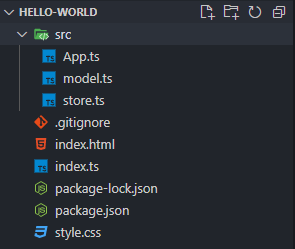
\includegraphics[width=0.4\textwidth]{slike/hello-world-direktorijum.PNG}
  \caption{Struktura direktorijuma nakon izvršenja komande \ref{cmd:npx}}
  \label{fig:hello-world-direktorijum}
\end{figure}
\noindent Kako bismo pokrenuli našu aplikaciju, potrebno je da se pozicioniramo u 
novonapravljeni direktorijum i instališemo neophodne \emph{npm}-pakete,
izvršavanjem komande:
\shellcmd{cd hello-world \&\& npm install}{cmd:npm-install-hello-world}
\pagebreak

\noindent
Nakon što se ova komanda uspešno izvrši, možemo da pokrenemo našu aplikaciju
komandom:
\shellcmd{npm run start}{cmd:npm-start}
Ukoliko pokretanje ove komande nije izbacilo grešku, konzola bi trebalo da nas 
obavesti da je server za razvoj pokrenut i da možemo da mu pristupimo na 
adresi \url{http://localhost:1234} (Konzolni odgovor \ref{konzola:npmstart})\\
\renewcommand\lstlistingname{Konzolni odgovor}
\begin{lstlisting}[style=shellStyle, caption={Konzolna poruka nakon pokretanja aplikacije}, label=konzola:npmstart]
> pure-framework-hello-world-app@1.0.0 start
> parcel index.html

Server running at http://localhost:1234
Built in 27ms
\end{lstlisting}
\renewcommand\lstlistingname{Primer koda}

\noindent Ukoliko u pregledaču otvorimo stranicu \url{http://localhost:1234},
trebalo bi da vidimo stranicu koja izgleda kao na slici \ref{fig:hello-world} 

\begin{figure}[!ht]
  \centering
  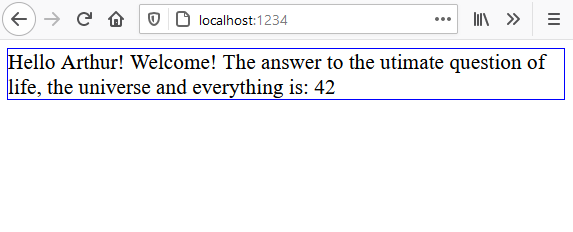
\includegraphics[width=0.7\textwidth]{slike/hello-world-strana.PNG}
  \caption{Aplikacija "Zdravo svete", pokrenuta na lokalnom serveru.}
  \label{fig:hello-world}
\end{figure}
\pagebreak

\subsection{Struktura aplikacije}
% Pogledajmo sada sadržaj fajlova koje smo napravili u koraku \ref{cmd:npx}.
% Primetićemo da fajlovi \code{index.html} i \code{index.ts} gotovo da ne sadrže
% nikakvu programsku logiku ili opis strukture DOM\footnote{ Document Object Model} drveta.
% U narednim poglavljima upoznaćemo se detaljnije sa svrhom ovih fajlova, ali ćemo
% te detalje za sada preskočiti.

\noindent Fajl koji sadrži centralnu logiku naše aplikacije je \code{src/App.ts} (Primer \ref{file:app.ts}).
\begin{lstlisting}[style=jsStyle, caption={Sadržaj fajla \code{App.ts}},label=file:app.ts]
import { Component, componentFactory } from "pure-framework/core";
import { div, span } from "pure-framework/html";
import { AppModel } from "./model";

class AppComponent extends Component<AppModel> {
  template() {
    return div({ class: 'app-root'}, [
      span(`Hello ${this.state.name}! Welcome! `),
      span(`The answer to the ultimate question of life, the universe and everything is: ${this.state.answer}`)
    ]);
  }
}
export const app = componentFactory(AppComponent);
\end{lstlisting}
\noindent
Ukoliko pogledamo aplikaciju u pregledaču (slika \ref{fig:hello-world})
videćemo da struktura HTML elemenata odgovara strukturi koju vraća funkcija \code{template()}.
Recimo da želimo da odredimo ponašanje našoj aplikaciji, tako da svaki put kada
kliknemo na element div povećamo broj iz pozdravne poruke za jedan, a ime promenimo u "Ford".
To možemo da uradimo tako što ćemo izmeniti funkciju \code{template()} na sledeći način:

\begin{lstlisting}[style=jsStyle, firstnumber=4, caption={Fajl \code{App.ts} nakon izmenjene funkcionalnosti},label=file:app.ts:2]
import { store } from "./store";|\Suppressnumber|
...|\Reactivatenumber{6}|
template() {
  return div({ class: 'app-root'}, [
    span(`Hello ${this.state.name}! Welcome! `),
    span(`The answer to the ultimate question of life, the universe and everything is: ${this.state.answer}`)
  ]).on('click', () => {
    store.updateState({
      answer: this.state.answer + 1,
      name: 'Ford'
    });
  });
}
\end{lstlisting}
\begin{figure}[!ht]
  \centering
  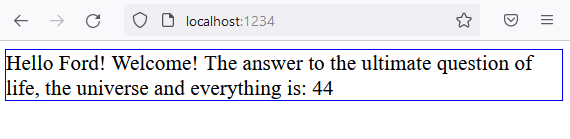
\includegraphics[width=0.7\textwidth]{slike/hello-ford.PNG}
  \caption{Aplikacija "Zdravo svete", nakon izmenjene funkcionalnosti.}
  \label{fig:hello-ford}
\end{figure}
\noindent
Ukoliko otvorimo ponovo našu aplikaciju u pregledaču i kliknemo na nju dva puta,
uočićemo da broj koji se prikazuje na kraju poruke više nije 42, već 44,
dok je pozdravna poruka ovog puta, umesto Arturu, namenjena Fordu (slika \ref{fig:hello-ford}).
\section{Struktura Pure-aplikacija}
Nakon pravljenja prvog programa u okruženju \emph{Pure}, pogledaćemo detaljnije strukturu i
značenje fajlova jedne \emph{Pure}-aplikacije oslanjajući se na primer aplikacije "Zdravo svete".
\subsection{Mesto povezivanja}\label{subsec:mesto-povezivanja}
Prvi fajl koji se učitava i izvršava, nakon fajla \code{index.html} je \code{index.ts} (Primer \ref{file:index.ts}).
Zbog toga u njemu pozivamo funkciju za povezivanje (eng. \emph{bootstrap}) aplikacije.
Metoda \code{bootstrap()} prihvata tri argumenta.
\begin{enumerate}
  \item Referencu na koreni element DOM-drveta aplikacije. To jest, element iz fajla \code{index.html} koji želimo da zamenimo \emph{Pure} aplikacijom;
  \item Konstruktorsku funkciju korene komponente napisane u okruženju \emph{Pure} i
  \item Referencu na objekat koji upravlja skladištem (eng. \emph{storage / store}).
\end{enumerate}
Treći argument se prosleđuje funkciji povezivanja kako bi okruženje moglo da osluškuje promene stanja
u objektu \code{store} i reaguje na te promene ponovnim iscrtavanjem elemenata DOM-a.
\begin{lstlisting}[style=jsStyle, caption={Fajl \code{index.ts}},label=file:index.ts]
import { bootstrap } from "pure-framework/core";
import { app } from "./src/App";
import { store } from "./src/store";

bootstrap(document.getElementById('app'), app, store);
\end{lstlisting}

\subsection{Komponente}
Komponente sadrže logiku i vizuelni opis dela aplikacije. Svaka komponenta u okruženju Pure
mora da nasledi apstraktnu klasu \code{Component<T>}, gde generički argument \code{<T>} predstavlja tip modela podataka komponente.
Konstruktor komponente ne treba pozivati neposredno, već je potrebno
napraviri posredničku funkciju (eng. \emph{proxy}) koju možemo napraviti pomoću funkcije \code{componentFactory} koja se uvozi sa putanje
\code{"pure-framework/core"}. Razlog za ovo, kao i detalji implementacije funkcije \code{componentFactory} biće pojašnjeni u kasnijim poglavljima.

Klasa \code{Component<T>} sadrži razne metode,
ali ćemo se u ovom delu fokusirati na dve: Metodu \code{template()} i metodu \code{render()}.

Metoda \code{template()} je apstraktna metoda koju mora da implementira
svaka komponenta koja nasleđuje klasu \code{Component<T>}. Ona je zadužena za pravljenje strukture DOM-elemenata komponente i po potpisu funkcije
mora da vrati objekat tipa \code{FunctionalElement}. Tip \code{FunctionalElement} je interfejs o kome će biti više reči kasnije,
ali je za sada dovoljno pomenuti da ovaj interfejs implementiraju sve klase iz
kolekcije ugrađenih funkcionalnih elemenata.

Primer jednog funkcionalnog elementa je instanca klase \code{DivElement}. Instance ovih klasa se nikada ne kreiraju neposredno pozivanjem konstruktora,
već isključivo korišćenjem specijalnih \emph{factory}-funkcija\footnote{\emph{Factory} - eng. Fabrika. U ovom kontekstu: "Obrazac Fabrika" - obrazac za kreiranje novih objekata.}.
Ovo je važno zbog iskorišćenja optimizacionih mehanizama okruženja, ali i zbog čitljivosti koda.

Važno je napomenuti
da i klasa \code{Component<T>} takođe implementira interfejs \code{FunctionalElement}, što znači da povratna vrednost metode \code{template()} takođe može biti i druga komponenta.
\subsection{Funkcionalni elementi}

Sve ugrađene \emph{factory}-funkcije za kreiranje funkcionalnih elemenata, koji služe opisu ugrađenih HTML-elemenata, mogu se uvesti sa putanje \code{"pure-framework/html"}.
Sve ugrađene \emph{factory}-funkcije ovih funkcionalnih elemenata imaju isti potpis.
Ove funkcije podrazumevano prihvataju dva argumenta:
\begin{enumerate}
  \item Objekat atributa. \label{enum:attr-list}
  \item Listu unutrašnjih elemenata. (Lista čvorova-dece)
\end{enumerate}
Važno je napomenuti da ukoliko se prosledi samo jedan argument, podrazumeva se da je u pitanju lista unutrašnjih elemenata,
a ne objekat atributa, jer je češći slučaj da HTML element nema definisane atribute, nego što je slučaj da nema podčvorove.
Ukoliko element sadrži samo jedan unutrašnji element, možemo i izostaviti pakovanje tog elementa u niz i pustiti da okruženje
to uradi umesto nas.
Svi ovi izuzeci dodati su u okruženje radi lakše čitljivosti i smanjenja suvišnog koda. U prikazima \ref{file:functionalElement} i \ref{file:htmlElement}
možemo videti kako se prevodi jedna
struktura funkcionalnih elemenata u HTML elemente.
\\
\\
\noindent\begin{minipage}[b]{.46\textwidth}
\begin{lstlisting}[style=jsStyle, numbers=left, numberstyle=\tiny, caption={Funkcionalni element},label=file:functionalElement]
div({ id: 'app-root',  }, [
  span('Some inline text'),
  span('More inline text'),
  div({ class: 'inner-div'}, [
    span([
      span('left text'),
      a({ href:'https://google.com' }, ['Link']),
      span('right text'),
    ])
  ])
]);
\end{lstlisting}
\end{minipage}
\hfill
\begin{minipage}[b]{.46\textwidth}
\begin{lstlisting}[style=htmlStyle, numbers=left, numberstyle=\tiny, caption={Rezultujući HTML},label=file:htmlElement]
<div id="app-root">
  <span>Some inline text</span>
  <span>More inline text</span>
  <div class="inner-div">
    <span>
      <span>left text</span>
      <a href="https://google.com"> Link </a>
      <span>right text</span>
    </span>
  </div>
</div>
\end{lstlisting}
\end{minipage}

\subsection{Model i skladište podataka}
Modeli u okruženju Pure ne sadrže nikakvu logiku i pišu se pomoću interfejsa u \emph{TypeScript}-u, tako da postoje samo u fazi razvoja.
U fazi izvršavanja, ovi fajlovi nisu deo izvornog koda, zato što se uklanjaju u postupku prevođenja.
Njihova svrha je samo da nam obezbede striktne tipove pri navođenju podrazumevanih vrednosti i spreče eventualne logičke greške u fazi izvršavanja.
Model skladišta za aplikaciju "Zdravo svete" može se videti na primeru \ref{file:model.ts}.
\begin{lstlisting}[style=jsStyle, caption={Fajl \code{src/model.ts}},label=file:model.ts]
export interface AppModel {
  name: string;
  answer: number;
} 
\end{lstlisting}
Skladište koje se koristi u okviru okruženja Pure zasnovano je na mehanizmu
\emph{BehaviorSubject}-a\footnote{\emph{BehaviorSubject} - eng. Subjekt ponašanja} iz biblioteke \emph{RxJs}. 
Kako bismo napravili jednu instacu skladišta za našu aplikaciju, potrebno je da pozovemo konstruktor \code{Store<T>}
koji moramo uvezemo sa putanje \code{"pure-framework/core"}. Konstruktor \code{Store<T>} prima jedan generički argument tipa modela,
i jedan standardni argument koji predstavlja objekat podrazumevanog stanja koji odgovara po svojoj strukturi prosleđenom generičkom argumentu (Primer \ref{file:store.ts}).

\begin{lstlisting}[style=jsStyle, caption={Fajl \code{src/store.ts}},label=file:store.ts]
import { Store } from "pure-framework/core";
import { AppModel } from "./model";

export const store = new Store<AppModel>({
    name: 'Arthur',
    answer: 42
})
\end{lstlisting}
\section{Aplikacija "Menadžer Zadataka"}
Pogledaćemo sada malo kompleksniji primer.
U pitanju je aplikacija za upravljanje dnevnim obavezama\footnote{\emph{eng. TO-DO} lista.}.
Veze ka online verziji ove aplikacije kao i izvorni k\^od mogu se naći u dodatku (Poglavlje \ref{chap:dodatak}).

\begin{figure}[!ht]
  \centering
  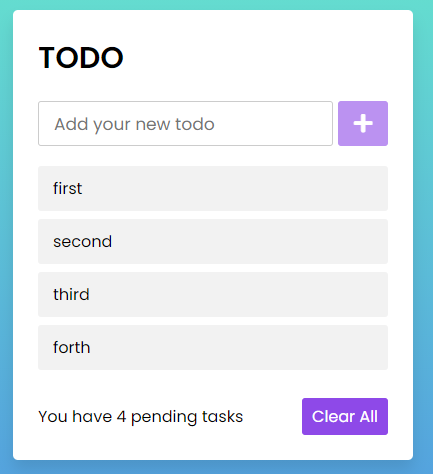
\includegraphics[width=0.3\textwidth]{slike/todo-app-online.PNG}
  \caption{Оnline verzija aplikacije "Menadžer zadataka"}
  \label{fig:todo-app}
\end{figure}
\pagebreak

\subsection{Struktura aplikacije}

Pogledajmo sada isečak koda koji odgovara korenoj komponenti \code{ToDoApp} koja se nalazi u fajlu \code{src/ToDoApp.ts}: 
\begin{lstlisting}[style=jsStyle, caption={Fajl \code{ToDoApp.ts}},label=file:ToDoApp.ts]
import { ... }; // Lista zavisnosti skracena zbog citljivosti |\Suppressnumber|
... |\Reactivatenumber{7}|
class ToDoApp extends Component<ToDoState> {|\Suppressnumber|
...|\Reactivatenumber{19}|
  template() {
    return div({ class: 'wrapper' }, [
      this.headerSegment(),
      this.todoSegment(),
      this.footerSegment(),
    ]);
  } |\Suppressnumber|
...|\Reactivatenumber{46}|
  private todoSegment() {
    return ul({ class: 'todoList' },[
      ...this.state.todoList.map((item) =>
        li([
          item,
          span({ class: 'icon' }, [
            italic({ class: 'fas fa-trash' }, [])
          ]).on('click', () => {
            let index = this.state.todoList.findIndex(x => x == item);
            this.state.todoList.splice(index, 1);
            store.updateState(this.state);
          })
        ]))
    ]);
  }|\Suppressnumber|
...|\Reactivatenumber{109}|
}

export const todoApp = componentFactory<ToDoApp, ToDoState>(ToDoApp);

\end{lstlisting}
\noindent
Ukoliko pogledamo strukturu liste potomaka u metodi \code{template()} (Primer \ref{file:ToDoApp.ts}) videćemo da ona upravo opisuje tri vizualna segmenta aplikacije \ref{fig:todo-app}:
\begin{enumerate}
  \item Zaglavlje sa naslovom, poljem za unos novog zadatka i dugmetom za potvrdu unosa (Funkcija \code{headerSegment()});
  \item Segment sa listom aktuelnih zadatka (Funkcija \code{todoSegment()}) i
  \item Podnožje sa prikazom zbirnih informacija i dugmetom za brisanje liste aktuelnih zadataka (Funkcija \code{footerSegment()}).
\end{enumerate}

\noindent
U primeru koda \ref{file:ToDoApp.ts} prikazan je k\^od funkcije koja opisuje deo aplikacije sa listom aktuelnih zadataka.
Funkcija \code{todoSegment()} vraća \code{UlElement} funckcionalni element (povratna vrednost \emph{factory}-funkcije \code{ul()}),
koji odgovara HTML-elementu \code{<ul>}).
U redu 48 vidimo poziv operatora \emph{spread (eng. raširi)} nad nizom koji se dobija kao rezultat mapiranja niza
\code{this.state.todoList} u niz elemenata \code{li}. Svaki od elemenata \code{li} takođe sadrži dva deteta-čvora, od kojih jedan
predstavlja nisku koja sadrži opis zadatka i dugme za uklanjanje zadatka.

Funkcija za uklanjanje pojedinačnih zadatka opisana je kodom koji počinje u redu 54, primera \ref{file:ToDoApp.ts}.
Primetimo bitan detalj u redu 56, u kojem pozivamo metodu nad objektom \code{store} sa novim, izmenjenim stanjem.
Ovaj poziv je neophodan kako bismo korenoj komponenti signalizirali promenu stanja aplikacije, i naterali okruženje da ponovo
izvrši iscrtavanje.

Ova veza između komponente \code{todoApp} i objekta \code{store} ostvarena je pozivanjem metode \code{bootstrap()} u fajlu \code{index.ts} (Primer \ref{file:index.ts}).
% \begin{lstlisting}[style=jsStyle, caption={Fajl \code{ToDoApp.ts}},label=file:index.ts]
% import { bootstrap } from "pure-framework/core";
% import { todoApp } from "./src/ToDoApp";
% import { store } from "./src/store";

% bootstrap(document.getElementById('app'), todoApp, store);
% \end{lstlisting}
Pogledajmo sada šta sadrži objekat \code{store}, koji uvozimo iz fajla \code{src/store.ts} (Primer \ref{file:todo-store.ts}).
\begin{lstlisting}[style=jsStyle, caption={Fajl \code{src/store.ts}},label=file:todo-store.ts]
import { Store } from "pure-framework/core";
import { ToDoState } from "./model";

export const store = new Store<ToDoState>({
  todoList: [
      'Kupi mleko',
      'Odvezi auto kod majstora',
      'Napisi master rad',
      'Odbrani master rad',
  ]
});
\end{lstlisting}
Na osnovu prikaza \ref{file:todo-store.ts} vidimo da je objekat \code{store} instanca klase \code{Store} koja je definisana u okviru paketa \code{pure-framework}.
Konstruktor ove klase prima generički argument (\code{ToDoState}) koji opisuje model podataka naše aplikacije (model podataka korene komponente) i inicijalizujući objekat,
koji se koristi kao podrazumevano stanje komponente ili u ovom slučaju cele aplikacije.

Model podataka aplikacije opisan je \emph{TypeScript}-interfejsom koji je definisan u fajlu \code{src/model.ts} (Primer \ref{file:todo-model.ts})
\begin{lstlisting}[style=jsStyle, caption={Fajl \code{src/model.ts}},label=file:todo-model.ts]
export interface ToDoState {
  todoList: string[];
}
\end{lstlisting}

\chapter{Implementacija okruženja Pure}\label{chap:pure-implementacija}
U ovom poglavlju upustićemo se u detalje implementacije okruženja \emph{Pure} i
objasniti neke odluke donete tokom dizajniranja samog okruženja.

\section{Korišćeni alati, tehnologije i biblioteke}
Za rešavanje većine problema opisanih u odeljcima \ref{problemi:ang} i \ref{problemi:react} postoje različiti alati i biblioteke. 
Kako bi fokus okruženja \emph{Pure} trebalo da bude na do sada nerešenim (ili nedovoljno adekvatno rešenim) problemima,
potrebno je odabrati i uvezati ove postojeće alate na pravi način. U ovoj sekciji ćemo opisati glavne
alate i biblioteke koje predstavljaju deo okruženja \emph{Pure}, ili su korišćene tokom razvoja okruženja.

\subsection{Typescript}
\emph{TypeScript} je strogo tipizirani programski jezik izgrađen oko jezika \emph{JavaScript}.
Prednost korišćenja strogih tipova u pisanju aplikacija leži u mogućnosti programskih alata
da veliki opseg grešaka otkriju u fazi razvoja. Primera radi, ukoliko neka funkcija kao ulazni
argument očekuje nisku,
a mi nad tim argumentom pozivamo metodu koja nije definisana na
prototipu\footnote{Sistem nasleđivanja u jeziku \emph{JavaScript}
je baziran na prototipovima \cite{PrototypeInheritance}.} niske,
kompilator će nam izbaciti grešku i upozoriti nas da to (verovatno) nije metoda koju smo želeli da pozovemo \cite{PrototypeInheritance}.

Pošto \emph{TypeScript} predstavlja suštinski samo nadskup jezika \emph{JavaScript} (korišćenje tipova je opciono),
možemo jednostavno balansirati između korišćenja striktnih tipova i sigurnosti sa jedne strane i jednostavnosti koda sa druge,
tako da je cena uvođenja ove tehnologije u okruženje veoma niska, a dobici mogu biti značajni.
\subsection{Parcel}
\emph{Parcel} je popularan upakivač (eng. \emph{bundler}) za veb aplikacije.
Upakivač u razvojnim okruženjima ima dva zaduženja:
\begin{enumerate}
  \item Pravljenje \emph{produkcionog} \emph{JavaScript} fajla sa minifikovanim kodom \cite{Minification}.
  \item Povezivanje koda i veb pregledača tokom pisanja koda.
\end{enumerate} 
\emph{"Produkcioni JavaScript fajl"} je fajl koji sadrži celokupnu logiku aplikacije, ali je za potrebe brzog preuzimanja i
učitavanja od strane pregledača minifikovan i preveden na nižu verziju standarda \emph{ECMAScript} \cite{ECMAScript} (zbog starijih verzija pregledača).
Ukratko, sve beline iz koda su uklonjene, a promenljive preimenovane u kraća simbolička imena. Napredni konstrukti jezika
prevode se na semantičke ekvivalente iz starije verzije \emph{ECMAScript}-a.

Glavna prednost upakivača \emph{Parcel} je u minimalnoj neophodnoj konfiguraciji.
Konkretan razlog zbog kog je \emph{Parcel} odabran kao upakivač, je taj što \emph{Parcel} automatski
prevodi \emph{TypeScript} k\^od na \emph{JavaScript} bez ikakvog dodatnog podešavanja, pa zbog toga možemo u okviru
fajla \code{index.html} neposredno da zahtevamo \emph{TypeScript} fajl (Primer \ref{file:html-Typescript}).
\begin{lstlisting}[style=htmlStyle,numberstyle=\tiny, caption={Uključivanje \emph{TypeScript} fajla neposredno u \code{index.html}}, label=file:html-Typescript]
<script src="index.ts" type="module"></script>
\end{lstlisting}
U ovom konkretnom primeru (Primer \ref{file:html-Typescript}), \emph{Parcel} će u pozadini prevesti \emph{TypeScript} k\^od na \emph{JavaScript}
i zameniti referencu ka \emph{TypeScript}-fajlu minifikovanim rezultujućim \emph{JavaScript}-fajlom u momentu upakivanja koda.
\subsection{RxJs}
\emph{RxJs} je biblioteka koja sadrži generičku implementaciju obrazca \emph{Observer}\footnote{\emph{Observer} - eng. Posmatrač.} za \emph{JavaScript} \cite{GoF,RxJs}.
Deo je većeg skupa alata otvorenog koda pod nazivom \emph{ReactiveX} koji služe reaktivnom programiranju \cite{ReactiveX}.

Reaktivno programiranje podrazumeva programiranje vođeno događajima. Popularna implementacija obrasca \emph{Redux} koja se koristi za \emph{Angular} aplikacije
pod nazivom \emph{NgRx} je implementirana upravo nad ovom bibliotekom \cite{Redux,NgRx}. Okruženje \emph{Pure} koristi
biblioteku \emph{RxJs} iz istih razloga, ali u značajno pojednostavljenoj varijanti.
\subsection{Ostali alati i biblioteke}
Pored glavnih alata opisanih u ovom poglavlju, korišćeni su i alati otvorenog koda za manje i jednostavnije zadatke.
Neki od njih su:
\begin{enumerate}
  \item \texttt{jest} - Okruženje za testiranje \emph{JavaScript} koda.
  \item \texttt{jsdom} - Implementacija pregledača i DOM-а u redukovanoj konzolnoj verziji zarad lakšeg automatskog testiranja.
  \item \texttt{object-hash} - Implementacija različitih heš algoritama za heširanje
  \emph{JavaScript} objekata, zarad brzog poređenja objekata po vrednosti.
  \item \texttt{rfdc} - Implementacija algoritma za \emph{duboko kloniranje}\footnote{Pri dubokom kloniranju reference ka pod-objektima se ne dele između originalnog i kloniranog objekta, već se svi pod-objekti takođe kloniraju.} \emph{JavaScript} objekata. 
\end{enumerate}

\section{Povezivanje}
Kao što je već pomenuto u sekciji \ref{subsec:mesto-povezivanja}, \code{index.ts} je prvi fajl
koji biva učitan nakon fajla \code{index.html}. Jedina funkcija koju pozivamo u ovom fajlu (u do sada prikazanim primerima)
je funkcija za povezivanje aplikacije: \code{bootstrap()}.
Njena implementacija nalazi se u fajlu \code{core/bootstrap.ts} i može se videti u primeru \ref{file:src:bootstrap.ts}.
\noindent
Funkcija \code{bootstrap()} je generička funkcija koja prihvata jedan argument, čiji tip
odgovara tipu korenog modela podataka, i tri standardna argumenta. Standardni argumenti su:
\begin{enumerate}
  \item Referenca na element DOM-a;
  \item Konstruktorska funkcija komponente i
  \item Referenca na objekat skladišta.
\end{enumerate}
Ovi argumenti su već opisani u sekciji \ref{subsec:mesto-povezivanja}, pa njihovo značenje nećemo ovde ponovo navoditi.
\begin{lstlisting}[style=jsStyle, caption={Fajl \code{core/bootstrap.ts}},label=file:src:bootstrap.ts]
import { Component } from "./component";
import { Store } from "./store";

export function bootstrap<AppModel>(
    domRoot: HTMLElement,
    rootComponentFactory: (state: () => AppModel) => Component<AppModel>,
    store: Store<AppModel>,
): Component<AppModel> {

    const appRoot = rootComponentFactory(() => store.state);
    store.state$.subscribe(state => {
        while (domRoot.firstChild) {
            domRoot.removeChild(domRoot.lastChild);
        }
        domRoot.appendChild(appRoot.render());
    });

    return appRoot;
}
\end{lstlisting}
Ukoliko bliže analiziramo prikazani k\^od, primetićemo da funkcija \code{bootstrap()} ima 3 zaduženja:
\begin{enumerate}
  \item Instanciranje korene komponente pozivom prosleđene \emph{factory}\footnote{\emph{Factory} - eng. Fabrika. U ovom konteksu "obrazac Fabrika" \cite{GoF}.}-funkcije (Linja 10) \cite{GoF}.
  \item Osluškivanje promene stanja skladišta (Linija 11).
  \item Registrovanje anonimne funkcije za ponovno iscrtavanje elemenata DOM-a (Linije 11-16).
\end{enumerate}
Iako će pojedinačni detalji komponenata, fabrike komponenata, skladišta i obrade događaja biti objašnjeni u kasnijim poglavljima,
ovde ćemo navesti neke važnije aspekte ovih elemenata, kako bismo jasnije razumeli prikazani k\^od. 

Primetimo da drugi argument koji prihvata funkcija \code{bootsrap()},
u samom kodu nazivamo \code{rootComponentFactory}. Razlog je u tome što prosleđena funkcija nije 
samo jednostavni konstruktor, već ima dodatnu funkcionalnost u domenu optimizacije.
U liniji 11 vidimo poziv metode \code{subscribe()} nad objektom \code{store.state\$}.
Ovo je metoda koja je definisana u okviru biblioteke \emph{RxJs} nad tipom \code{Observable<T>.} Više detalja o ovom
i drugim tipovima iz biblioteke \emph{RxJs} biće u odeljku \ref{sec:promena-stanja}.


\section{Funkcionalni Elementi}
Tip \code{FunctionalElement} predstavlja interfejs najopštijeg nivoa u hijerarhiji strukturnih
elemenata okruženja \emph{Pure}\footnote{Elementi za opis DOM-strukture.},
koji sadrži minimalan skup metoda koje se podrazumevano mogu pozvati nad bilo kojim elementom.
U kodu je definisan \emph{TypeScript} interfejsom na putanji \code{core/functionalElement.ts}
(Primer \ref{file:core:functionalElement.ts}).
\begin{lstlisting}[style=jsStyle, escapeinside=\#\#, caption={Fajl \code{core/functionalElement.ts}},label=file:core:functionalElement.ts]
export interface FunctionalElement {
  render: () => HTMLElement;
  domElement: HTMLElement;
  children?: FunctionalElement[];
  parentDomElement: HTMLElement;
}

\end{lstlisting}
Interfejs \code{FunctionalElement} deklariše sledeće metode i polja:
\begin{enumerate}
\item Metodu \code{render()} koja se poziva pri iscrtavanju DOM-elemenata;
\item Referencu na DOM-element koji napravljen pozivanjem metode \code{render()};
\item Listu potomaka i
\item Referencu na "roditelja" DOM-elementa (\code{null} u slučaju korene komponente).
\end{enumerate}
  
Primetimo da prikazani interfejs (Primer \ref{file:core:functionalElement.ts}) pored metode (\code{render()}) sadrži i polja.
Ovo je specifično za jezik \emph{TypeScript} u kojem interfejsi mogu definisati i polja, a ne samo metode\footnote{Pošto neposredno pristupanje poljima instance nije redak slučaj u \emph{JavaScript}-u, inženjeri
\emph{TypeScript}-a su odlučili da zvanično tako nešto podrže i u svojoj sintaksi.}.
\subsection{Ugrađeni Funkcionalni Elementi}
Kako bismo izgradili nove komponente koristeći obrazac kompozicije (eng. \emph{Composite pattern}),
moramo se osloniti na neke postojeće, to jest, elemente ugrađene u okruženje.
Elementi koji su ugrađeni u okruženje \emph{Pure} su elementi koji predstavljaju pandan postojećim HTML elementima
(\code{div}, \code{h1}, \code{span}, ...).

U nastavku poglavlja prikazaćemo implementaciju funkcionalnog elementa \code{div} kao i dijagram klasa koji
opisuje hijerarhiju i odnose elementa \code{div} sa ostalim elementima.
Implementacija ostalih funkcionalnih elemenata može se naći na repozitorijumu okruženja \emph{Pure}.

\begin{figure}[!ht]
  \centering
  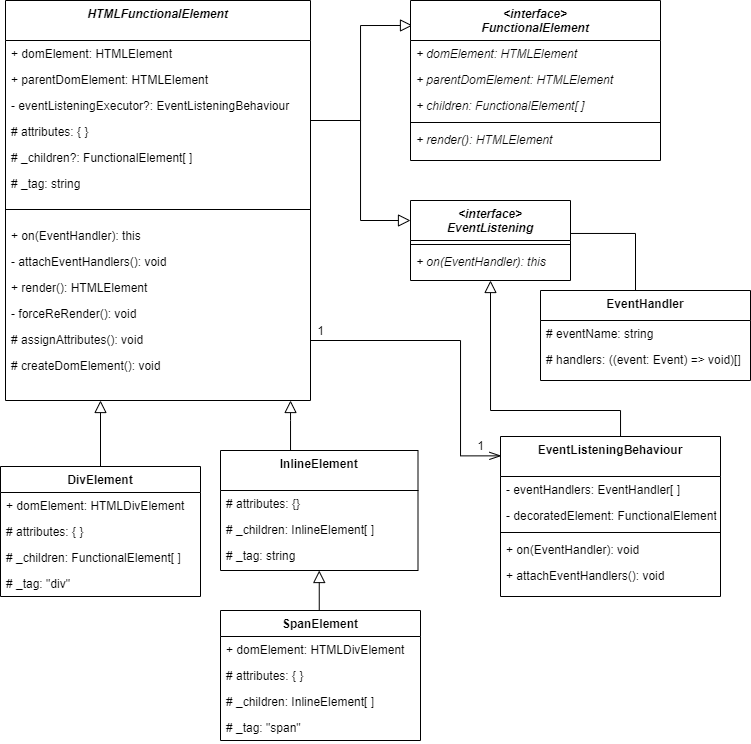
\includegraphics[width=0.8\textwidth]{slike/HTMLFunctionalElement_dijagram.drawio.png}
  \caption{Dijagram klasa za klasu \code{HTMLFunctionalElement}}
  \label{fig:dijagram-klasa-HTMLFunctionalElement}
\end{figure}
\pagebreak

\noindent
Na osnovu dijagrama (slika \ref{fig:dijagram-klasa-HTMLFunctionalElement}) vidimo da \code{DivElement} nasleđuje
klasu \\\code{HTMLFunctionalElement}.
Ukoliko pogledamo k\^od klase \code{DivElement} (Primer \ref{file:html:blockElements:divElement.ts}) primetićemo da klasa \code{DivElement}
ne dodaje nikakvo ponašanje u odnosu na klasu \code{HTMLFunctionalElement}, osim što fiksira argument imena elementa (\code{\_tag}).

\begin{lstlisting}[style=jsStyle, escapeinside=\#\#, caption={Fajl \code{html/block/elements/divElement.ts}},label=file:html:blockElements:divElement.ts]
import { FunctionalElement, HTMLFunctionalElement } from '/core';
export class DivElement extends HTMLFunctionalElement {
    constructor(protected attributes: {}, protected _children: FunctionalElement[]) {
        super(attributes, _children, 'div')
    }
}
\end{lstlisting}

Kao što se da zaključiti iz njenog naziva, \code{HTMLFunctionalElement} je klasa koja definiše ponašanje svih ugrađenih
elemenata HTML-a.
Pogledajmo sada detalje implementacije klase \code{HTMLFunctionalElement}:

\begin{lstlisting}[style=jsStyle, escapeinside=\#\#, caption={Fajl \code{core/htmlFunctionalElement.ts}},label=file:core:HTMLFunctionalElement.ts]
import { EventListening } from "./eventListening";
import { EventListeningBehaviour } from "./eventListeningBehaviour";
import { FunctionalElement } from "./functionalElement";

export abstract class HTMLFunctionalElement implements FunctionalElement, EventListening {
  public domElement: HTMLElement;
  public parentDomElement: HTMLElement;
  private _eventListeningExecutor: EventListeningBehaviour = null;

  constructor(protected attributes: {}, protected _children: FunctionalElement[], protected _tag: string) {
    // logic for handling order of parameters excluded for brevity
    this._eventListeningExecutor = new EventListeningBehaviour(this);
  }

  public on(event: string, ...handlers: ((event: Event) => void)[]) {
    this._eventListeningExecutor.on(event, ...handlers);
    return this;
  }

  public get children(): (FunctionalElement)[] {
    return this._children;
  }

  public render(): HTMLElement {
    this.createDomElement();
    this.assignAttributes();
    this.attachEventHandlers();
    return this.domElement;
  }

  public forceReRender() {
    let domElementToReplace = this.domElement;
    this.parentDomElement.replaceChild(this.render(), domElementToReplace);
  }

  protected assignAttributes(): void {
    Object.keys(this.attributes).forEach(attribute => {
      if (this.attributes[attribute]) {
        this.domElement.setAttribute(attribute, this.attributes[attribute]);
      }
    });
  }

  protected createDomElement(): void {
    this.domElement = document.createElement(this._tag);

    this.children.forEach(child => {
      child.parentDomElement = this.domElement;
      this.domElement.appendChild(child.render());
    });
  }

  private attachEventHandlers() {
    this._eventListeningExecutor.attachEventHandlers();
  }
}

\end{lstlisting}
Metoda \code{render()} klase \code{HTMLFunctionalElement} interno poziva tri privatne metode:
\begin{enumerate}
  \item Metodu za pravljenje elementa DOM-a (\code{createDomElement()});
  \item Metodu za dodeljivanje potencijalno prosleđenih atributa napravljenom DOM-elementu (\code{assignAttributes()}) i
  \item Metodu za registraciju osluškivača događaja (\code{attachEventHandlers()}).  
\end{enumerate}
U privatnoj metodi \code{createDomElement()}, nakon samog poziva za kreiranje DOM-elemenata se proverava
da li je funkcionalnom elementu prosleđena lista potomaka. Ukoliko jeste, metoda iterira kroz tu listu i rekurzivno
za svako dete poziva metodu \code{render()} i na taj način se formira celo drvo DOM-elemenata (Primer \ref{file:core:HTMLFunctionalElement.ts}, Linije 54-63).

Privatna metoda \code{assignAttributes()} prolazi kroz listu atributa koje imaju vrednost
\emph{truthy}\footnote{Skup vrednosti u \emph{JavaScript}-u koje se konverzijom prevode na \emph{boolean} vrednost \texttt{true} \cite{Truthy}.}
i dodeljuje prosleđene atribute DOM-elementu.

Mehanizam registrovanja osluškivača događaja i samo upravljanje događajima biće obrađeno u sekciji \ref{sec:promena-stanja}.


\section{Komponente}
Komponente u okruženju \emph{Pure} predstavljaju funkcionalne elemente koji se mogu dinamički menjati
u odnosu na promenu stanja skladišta. Sve komponente moraju da naslede apstraktnu klasu \code{Component<T>}.
Ova apstraktna klasa ima jednu apstraktnu metodu \code{template()} koja se mora definisati u potklasi.

Metoda \code{template()} mora da vrati tip koji implementira interfejs \code{FunctionalElement}.
To može biti druga komponenenata ili neki od ugrađenih funkcionalnih elemenata.

Pošto klasa \code{Component<T>} implementira interfejs \code{FunctionalElement}, mora da implementira i metodu \code{render()}.
Metoda \code{render()} najpre proverava da li je stanje promenjeno u odnosu na prethodno i ukoliko nije,
vraća DOM-element koji je napravljen u prethodnom pozivu. Ukoliko je stanje promenjeno, trenutno stanje se čuva 
(kako bi moglo da se uporedi sa budućim), a nad objektom koji vraća metoda \code{template()} se poziva metoda \code{render()}.
Rezultat tog poziva se vraća kao izlazna vrednost metode \code{render()}.
\begin{figure}[!ht]
  \centering
  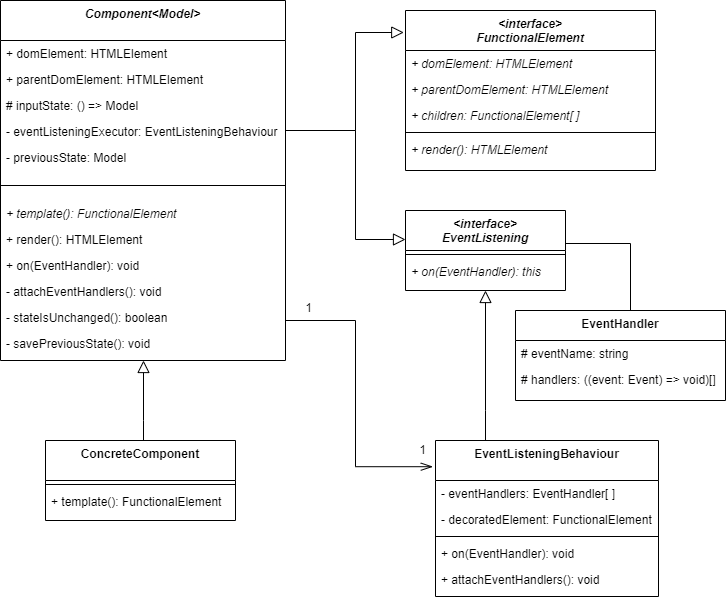
\includegraphics[width=0.8\textwidth]{slike/Component_dijagram.drawio.png}
  \caption{Dijagram klasa za klasu \code{Component<Model>}}
  \label{fig:dijagram-klasa}
\end{figure}
\\
\pagebreak

\noindent
Pogledajmo sada implementaciju klase \code{Component<T>}:
\begin{lstlisting}[style=jsStyle, escapeinside=\#\#, caption={Fajl \code{core/component.ts}},label=file:core:component.ts]
import { FunctionalElement } from "./functionalElement";
import { EventListeningBehaviour } from "./eventListeningBehaviour";
import { areEqual, cloneDeep } from "../utils";
import { EventListening } from "./eventListening";

export abstract class Component<ModelType>  implements FunctionalElement, EventListening {
    public domElement: HTMLElement | Text = null;
    public parentDomElement: HTMLElement = null;
    protected inputState: () => ModelType = () => null;
    private _eventListeningExecutor: EventListeningBehaviour = null;
    private previousState: ModelType = null;

    constructor(inputState: () => ModelType) {
        this._eventListeningExecutor = new EventListeningBehaviour(this);
        this.inputState = inputState;
    }

    abstract template(): FunctionalElement;

    get state() {
        return this.inputState();
    }

    get children() {
        return this.template().children
    }

    public render() {
        if (this.stateIsUnchanged() && this.domElement) {
            return this.domElement;
        }

        this.savePreviousState();
        this.domElement = this.template().render();
        this.attachEventHandlers();

        return this.domElement;
    }

    public on(event: keyof HTMLElementEventMap, ...handlers: ((event: Event) => void)[]) {
        this._eventListeningExecutor.on(event, ...handlers);
        return this;
    }

    private attachEventHandlers() {
        this._eventListeningExecutor.attachEventHandlers();
    }
    
    private stateIsUnchanged() {
        return areEqual(this.inputState(), this.previousState);
    }

    private savePreviousState() {
        this.previousState = cloneDeep(this.inputState());
    }
};

\end{lstlisting}

\section{Obrada događaja}
Obratimo pažnju na pojedine elemente na dijagramu klasa koji opisuje okruženje klase
\code{Component<Model>} i dijagramu klasa koji opisuje okruženje klase \code{HTMLFunctionalElement}.
Videćemo da pored osnovnog interfejsa svih elemenata (\code{FunctionalElement})
obe klase implementiraju interfejs \code{EventListening} i sadrže instancu klase koja neposredno implementira ovaj interfejs
(\code{EventListeningBehaviour}). Razlog za ovo je potreba za razdvajanjem interfejsa (eng. \emph{Interface Segregation})
i lakšim razvojem koda kroz princip \emph{"kompozicija ispred nasleđivanja"} (eng. \emph{Composition over Inheritance}).

Koriščenjem (pojednostavljenog) obrazca \emph{Dekorator} \cite{GoF} razdvajamo implementaciju za osluškivanje i
reagovanje na korisničke događaje.

Pogledajmo detalje ovog interfejsa, kao i konkretnu implementaciju (ista implementacija interfejsa se koristi i za \code{HTMLFunctionalElement} i za \code{Component<Model>}):
\begin{lstlisting}[style=jsStyle, escapeinside=\#\#, caption={Fajl \code{core/eventListening.ts}},label=file:core:eventListening.ts]
export interface EventListening {
  on: (event: keyof HTMLElementEventMap, ...handlers: ((event: Event) => void)[]) => this,
}
\end{lstlisting}
\begin{lstlisting}[style=jsStyle, escapeinside=\#\#, caption={Fajl \code{core/eventListeningBehaviour.ts}},label=file:core:eventListeningBehaviour.ts]
import { EventListening } from "./eventListening";
import { FunctionalElement } from "./functionalElement";

export class EventListeningBehaviour implements EventListening {
  private eventHandlers: { event: keyof HTMLElementEventMap; handlers: ((event: any) => any)[]; }[] = [];
  constructor(private decoratedElement: FunctionalElement) { }

  public on(event: keyof HTMLElementEventMap, ...handlers: ((event: Event) => void)[]) {
    this.eventHandlers.push({event, handlers});
    return this;
  };

  public attachEventHandlers(): void {
    if (this.eventHandlers) {
        this.eventHandlers.forEach(event => {
            event.handlers.forEach(handler => {
              this.decoratedElement.domElement.addEventListener(event.event, handler);
            });
        });
    }
  }
}
\end{lstlisting}
Obratimo sada pažnju na isečak koda iz implementacije klase \code{Component<T>} koji smo videli u primeru \ref{file:core:component.ts}:
\begin{lstlisting}[style=jsStyle, caption={Isečak koda iz fajla \code{core/component.ts}},label=file:core:component-partial.ts]
import { ... } from "..."; |\Suppressnumber|
  ... |\Reactivatenumber{15}|
    constructor(inputState: () => ModelType) {
        this._eventListeningExecutor = new EventListeningBehaviour(this);
        this.inputState = inputState;
    } |\Suppressnumber|
  ...|\Reactivatenumber{42}|
    public on(event: keyof HTMLElementEventMap, ...handlers: ((event: Event) => void)[]) {
        this._eventListeningExecutor.on(event, ...handlers);
        return this;
    }

    private attachEventHandlers() {
        this._eventListeningExecutor.attachEventHandlers();
    } |\Suppressnumber|
  ...|\Reactivatenumber{58}|
};

\end{lstlisting}
U primerima \ref{file:core:eventListeningBehaviour.ts} i \ref{file:core:component-partial.ts}
vidimo mehanizam delegacije ponašanja pri implementiranju interfejsa.
Naime, pošto suštinski i komponente i ugrađeni funkcionalni elementi reaguju na događaje na gotovo isti način,
ima smisla to ponašanje definisati u okviru posebne klase koju ne mora nasleđivati ni jedna od ove dve klase.
Na taj način činimo strukturu koda prilagodljivom budućim promenama u hijerarhiji klasa.

Klasa \code{EventListeningBehaviour} ima za cilj da dekoriše funkcionalni element
metodama \code{on()} i \code{attachEventHandlers()}.
\section{Promena stanja}\label{sec:promena-stanja}
Pogledajmo sada malo detaljnije kako \emph{Pure}-aplikacija implementira mehanizam skladišta, analizirajući k\^od iz primera \ref{file:core:store.ts}:
\begin{lstlisting}[style=jsStyle, escapeinside=\#\#, caption={Fajl \code{core/store.ts}},label=file:core:store.ts]
import { BehaviorSubject } from "rxjs";

export class Store<Model> {
    private _stateSubject: BehaviorSubject<Model>;

    constructor(defaultState: Model) {
        this._stateSubject = new BehaviorSubject(defaultState);
    }

    updateState(newState: Partial<Model>) {
        this._stateSubject.next({...this._stateSubject.getValue(), ...newState });
    }

    get state() {
        return this._stateSubject.getValue();
    }

    get state$() {
        return this._stateSubject.asObservable();
    }
}
\end{lstlisting}
Skladište u razvojnom okruženju \emph{Pure} se zasniva na tipu \code{BehaviorSubject<T>}
iz biblioteke \emph{RxJs}. \code{BehaviorSubject<T>} je klasa koja objedinjuje posmatrača i subjekta posmatranja
u obrazcu \emph{Observer}\footnote{\emph{Observer} - eng. Posmatrač} \cite{GoF}. Drugim rečima, nad objektom tipa
\code{BehaviorSubject<T>} možete da registruje
funkciju za obradu događaja pri promeni stanja, ali i
pozvati metodu za promenu stanja.
\begin{lstlisting}[style=jsStyle, escapeinside=\#\#, caption={Primer registrovanja osluškivača stanja},label=example:behaviorSubject.subscribe]
behaviorSubject.subscribe(newState => { /* handling new state */});
\end{lstlisting}
\begin{lstlisting}[style=jsStyle, escapeinside=\#\#, caption={Primer emitovanja novog stanja},label=example:behaviorSubject.next]
behaviorSubject.next({...oldState, changedProperty: 'new value'});
\end{lstlisting}
Ovaj mehanizam omogućava nam implementaciju centralizovanog sistema za skladištenje podataka.
Ako pogledamo k\^od konkretne implementacije skladišta \ref{file:core:store.ts}, videćemo da klasa ima jednu javnu metodu i dva javna svojstva:
\begin{enumerate}
  \item Svojstvo nad kojim vršimo registraciju osluškivača (\code{state\$});
  \item Svojstvo za vraćanje trenutnog stanja (\code{get state()}) i
  \item Metodu za promenu stanja (\code{updateState()}).
\end{enumerate}
Važno je napomenuti da će se svakim pozivom metode \code{updateState()}, interno stanje skladišta promeniti. To jest,
nakon svakog poziva metode \code{updateState()}, pozivanje svojstva \code{get state()} vratiće novi objekat.
To nam garantuje da osnovni princip obrasca \emph{Flux} neće biti narušen.
\section{Memoizacija}
Već smo napomenuli da se komponente nikada ne instanciraju neposredno preko svojih konstruktora,
već isključivo preko \emph{factory}-funkcija koje možemo napraviti koristeći ugrađenu funkciju \code{componentFactory}
koju možemo uvesti sa putanje \code{"pure-framework/core"} (Primer \ref{file:core:componentFactory.ts}).
Razlog za to leži u mehanizmu optimizacije implementiranom u okruženju \emph{Pure},
koji se bazira na principu memoizacije čistih funkcija \cite{functionalProgramming}.

\emph{Memoizacija} je mehanizam koji podrazumeva keširanje rezultata izlaznih vrednosti čistih funkcija,
po ključu koji se gradi od ulaznih parametara funkcije. Za implementaciju ovog mehanizma, neophodno je
da funkcije budu "čiste", to jest, da za iste ulazne parametre uvek proizvode isti izlazni rezultat.
\pagebreak

\noindent
Pogledajmo konkretnu implementaciju ovog mehanizma u funkciji\\\code{componentFactory} u primeru \ref{file:core:componentFactory.ts}\footnote{Imena tipova i promenljivih su skraćeni, radi preglednijeg preloma teksta.}:

\begin{lstlisting}[style=jsStyle, escapeinside=\#\#, caption={Fajl \code{core/componentFactory.ts}},label=file:core:componentFactory.ts]
import oh from 'object-hash';
import { Component } from './component';
type FuncCompConstr<ModelType> = { new(state: () => ModelType): Component<ModelType>; }

const dictionary = Object.create(null);

export function componentFactory<ConcreteComponent extends Component<ModelType>, ModelType>(constrFunc: FuncCompConstr<ModelType>)
    : (state: () => ModelType, id?: number | string) => ConcreteComponent {
    return (state: () => ModelType, id: number | string = 0) => {
        const stateHash = oh.MD5(state());
        const key = `${stateHash}_${id}`
        if (!dictionary[constrFunc.name]) {
            dictionary[constrFunc.name] = Object.create(null)
        }
        if (!dictionary[constrFunc.name][key]) {
            dictionary[constrFunc.name][key] = new constrFunc(state);
        }
        return dictionary[constrFunc.name][key] as ConcreteComponent;
    };
};
\end{lstlisting}
Funkcija \code{componentFactory()} je funkcija višeg reda. To znači da je povratna vrednost ove funkcije druga funkcija.
Vraćena funkcija ima potpis koji prihvata dva argumenta:
\begin{enumerate}
  \item Funkciju za izračunavanje trenutnog stanja (\code{state: () => ModelType}) i
  \item Opcioni identifikator komponente (\code{id?: number | string}).
\end{enumerate}
U liniji 5 primera \ref{file:core:componentFactory.ts} vidimo inicijalizaciju jednog rečnika (praznog objekta).
Ovaj rečnik služi kao keš mehanizam za korisnički definisane komponente. Taj mehanizam funkcioniše na sledeći način:
\begin{enumerate}
  \item Hešira trenutno stanje komponente koje se dobija pozivanjem funkcije \code{state()};
  \item Heš kodu se dodaje opcioni identifikator komponente i tako spojeni čine ključ rečnika \code{dictionary};
  \item Proverava se da li u rečniku postoji objekat sa tim ključem;
  \item Ukoliko ne postoji pravi se nova instanca komponente pozivanjem prosleđenog konstruktora i čuva se u rečniku pod izračunatim ključem. Novonapravljena instanca se vraća kao rezultat funkcije;
  \item Ukoliko postoji vraća se instanca iz rečnika.
\end{enumerate}

Opcioni identifikator komponente (\code{id}) služi za (retke) slučajeve kada dve iste komponente koristimo
na dva različita mesta u aplikaciji sa potpuno istim stanjem. U slučaju nedodavanja ovog identifikatora, ovaj mehanizam bi napravio samo jednu instancu komponenente umesto dve koliko je potrebno.
\chapter{Diskusija}\label{chap:diskusija}
U ovom poglavlju ćemo analizirati ispunjenost postavljenih zahteva i razmotriti moguća poboljšanja datog rešenja.
\section{Analiza ispunjenosti zahteva}
\noindent Osvrnimo se još jednom na listu zahteva iznetu u sekciji \ref{sec:zahtevi}:

Zahtev \ref{zahtev:1}, koji se odnosi na (ne)korišćenje
specijalizovanih sintaksi koje se prevode na HTML, ispunjen je
korišćenjem koncepta funkcionalnih elemenata. Umesto opisa HTML
strukture korisnik pozivom funkcija (fabričkih konstruktora
funkcionalnih elemenata) opisuje strukturu DOM-drveta i na taj način
koristi sve benefite statičke provere ispravnosti, sintaksnog
obeležavanja, lakog refaktorisanja i svega ostalog što jedan moderan
programski jezik podrazumevano donosi.

Napomenimo da uvođenje koncepta funkcionalnih elemenata pored pomenutih
benefita donosi i dodatnu kompleksnost. Kada programer
želi da iskoristi neki već postojeći HTML segment iz druge stranice,
k\^od napisan u HTML-u mora biti preveden
na funkcionalne elemente, iliti na \emph{TypeScript} k\^od,
kako bi taj segment mogao biti iskorišćen.

Zahtev \ref{zahtev:2}, koji se odnosi na implementaciju obrasca
\emph{Flux} ispunjen je implementacijom \code{Store<Model>}
mehanizma za skladištenje podataka. Podaci se (podrazumevano) kreću
u jednom smeru kroz aplikaciju koristeći obrazac \emph{Posmatrač}
implementiran u biblioteciji \emph{RxJs}.

Zahtev \ref{zahtev:3}, koji se odnosi na uočavanje grešaka u fazi razvoja ostvaren je statičkim tipovima i korišćenjem jezika \emph{TypeScript}.

Objavljivanjem paketa u javni \emph{npm}-registar, ispunjen je i zahtev \ref{zahtev:4}.

Zahtev \ref{zahtev:5}, koji se odnosi na otvorenost za modifikaciju,
ostvaren je objavljivanjem repozitorijuma pod licencom MIT \cite{MIT}.

Zahtev \ref{zahtev:6}, koji se odnosi na lako čitljivu strukturu
ostvaren je minimalnim kodom neophodnim za funkcionisanje
aplikacije, na sličan način na koji je to rešeno i u okruženju
\emph{React}. Jedina obavezna metoda u okviru implementacije jedne
komponente je metoda \code{template()}, koja definiše HTML
strukturu komponente. Sve ostale metode su opcione, pa korisnik ima
široku kontrolu nad organizacijom svog koda.

\section{Prostor za unapređenja}
Okruženje \emph{Pure} ima za cilj da adresira neke od problema koji
su prisutni u popularnim okruženjima za razvoj klijentskih veb aplikacija.
Kao takavo, više predstavlja dokaz koncepta (eng. \emph{Proof of Concept}),
nego rešenje spremno za komercijalnu upotrebu. Ono predstavlja
osnovu jednog kompletnijeg i robustnijeg okruženja, koje će
moći da se razvije na temeljima trenutnog rešenja.

Kao potencijalna
poboljšanja trenutnog rešenja, autor ovog rada vidi u unapređenju
strukture koda, dodavanju funkcionalnosti i podeli rešenja na manje
funkcionalne celine. U ovoj sekciji ćemo obrazložiti neke od tih
ideja.
\subsection{Struktura koda}
Kako bi trenutno rešenje moglo dalje da se razvija i napreduje u
okviru zajednice otvorenog koda, neophodno je najpre detaljno
dokumentovati i opisati različite modele upotrebe trenutno
postojećeg rešenja. Jedan deo tog posla sastoji se od dodavanja
\emph{JSDoc} komentara na sve javne metode koje se pozivaju iz
korisničkog okruženja u okviru razvoja jedne
\emph{Pure}-aplikacije \cite{JSDoc}. Drugi deo odnosi se na refaktorisanje
trenutnog rešenja i prelazak sa modela nasleđivanja na model
kompozicije klasa i ekstenzjiju specifičnih ograničenja za ugrađene
funkcionalne elemente, kako bi iskustvo pisanja koda bilo što lakše,
a potencijalne greške lako uočljive.

\subsection{Detaljnije automatsko testiranje}
Iako su osnovni automatski testovi za proveru najvažnijih
funkcionalnosti okruženja već napisani, oni se ne pokreću
automatski i ciljaju veoma uzan skup funkcionalnosti. Ovaj skup
testova bi trebalo proširiti i uvesti princip kontinualne
integracije i kontinualnog isporučivanje u proces.

\subsection{Proširenje funkcionalnosti}
Mnoge funkcionalnosti koje su deo prikazanih okruženja, nisu implementirane u okruženju
\emph{Pure}. Jedna od većih funkcionalnosti koja nedostaje je rutiranje.
Takođe, dobar deo ugrađenih HTML elemenata
nemaju svoju implementaciju u okviru okruženja \emph{Pure}. Autor se nada da će barem deo
ovih nedostataka biti rešen u budućnosti kroz zajednicu otvorenog koda.

\subsection{Proširenje obrasca Flux na obrazac CQRS}
Obrazac Flux implementiran u okruženju \emph{Pure} predstavlja jednu
pojednostavljenu verziju bez okidanja akcija i funkcije
\emph{skupljača}. Umesto jedne centralizovane funkcije skupljača,
okruženje \emph{Pure} ostavlja odgovornost nenarušavanja
konzistentnosti skladišta programerima.

Ovaj mehanizam može da se proširi do obrasca CQRS\footnote{CQRS - Command Query Responsibility Segregation \cite{CQRS}} \cite{CQRS} koji bi povećao
kompleksnost aplikacija sa jedne strane, ali bi omogućio lakše
skaliranje aplikacije u smislu kompleksnosti programskog koda.

Obrazac CQRS ima za cilj da u potpunosti odvoji k\^od koji utiče na
promenu stanja skladišta i koda koji samo čita trenutno stanje.
Specifičan je u odnosu na obrazac \emph{Flux} po tome što padrazumeva i čuvanje redosleda i detalja izvršenih komandi koje menjaju stanja što omogućava repliciranje svakog stanja aplikacije
do kog može da se stigne od početnog. Ovaj mehanizam je veoma značajan u pronalaženju eventualnih grešaka u kodu.
\subsection{Alat za prevođenje HTML-a}
Glavnu prepreku za korišćenje novog okruženja u odnosu na postojeće je korišćenje \emph{TypeScript} sintakse umesto HTML-a. Iako ovo ima svojih prednosti koje su već opisane u odeljku \ref{subsec:zasto-ne-html}, postoji veliki broj postojećih komponenti
napisanih u HTML-u, koje je nema razloga pisati ponovo.
Alat koji bi prevodio HTML sintaksu u funkcionalne komponente olakšao bi korišćenje okruženja \emph{Pure} programerima koji žele da koriste postojeće komponente napisane u HTML-u.

% ali i pokretanje online veb prezentacije za
% promociju i neformalnu dokumentaciju okruženja.

\chapter{Zaključak}\label{chap:zakljucak}

U ovom radu predstavljen je razvoj jednog modernog okruženja za razvoj klijentskih veb aplikacija. Pored toga, data je kratka analiza problema postojećih rešenja i najčešćih arhitekturalnih obrazaca.

U okviru rada nalaze se obrazloženja za odabir konkretnih alata i biblioteka, primeri korišćenja okruženja za pravljenje aplikacija kao i objašnjenje implementacije najvažnijih elemenata okruženja.

Ne postoji idealan softver i ne postoji idealno razvojno okruženje. Svaki izbor alata se uvek svodi na optimizaciju jednog skupa kvalitativnih atributa po cenu nekog drugog. Okruženje \emph{Pure} u ovom smislu nije izuzetak.
Zbog velikog broja biblioteka i okruženja u ekosistemu \emph{JavaScript} jezika, autor ne očekuje da će se rešenje koristiti u komercijalne svrhe,
ali se nada da će ovo rešenje, ili barem neki njegovi delovi, poslužiti kao inspiracija nekim budućim bibliotekama i okruženjima.
Okruženje razvijeno u okviru ovog rada objavljeno je pod licencom MIT \cite{MIT}, što znači da je otvoreno za modifikaciju i korišćenje u akademske ili komercijalne svrhe.
% % primer liste
% Можемо правити и набрајања:
% \begin{enumerate}
% \item Анализа 1
% \item Линеарна алгебра
% \item Аналитичка геометрија
% \item Основи програмирања
% \end{enumerate}


\chapter{Dodatak}
\label{chap:dodatak}
Resursi na mreži koji se prilažu uz tekst rada:
\begin{itemize}
  \item Repozitorijum okruženja \emph{Pure}: \url{https://github.com/maleksandar/pure-framework}
  \item Stranica \emph{npm}-paketa "pure-framework": \url{https://www.npmjs.com/package/pure-framework}
  \item Repozitorijum aplikacije "Zdravo svete!": \url{https://github.com/maleksandar/pure-framework-hello-world-app}
  \item Repozitorijum aplikacije "Menadžer zadataka": \url{https://github.com/maleksandar/pure-framework-todo-app}
  \item Online verzija aplikacije "Menadžer zadataka": \url{https://pure-framework-todo-demo.netlify.app/}
\end{itemize}
% ------------------------------------------------------------------------------
% Literatura
% ------------------------------------------------------------------------------
\literatura

% ==============================================================================
% Završni deo teze i prilozi
\backmatter
% ==============================================================================

% ------------------------------------------------------------------------------
% Biografija kandidata
% \begin{biografija}
% \textbf{Вук Стефановић Караџић} (\emph{Тршић, 26. октобар/6. новембар
%   1787. — Беч, 7. фебруар 1864.}) био је српски филолог, реформатор
% српског језика, сакупљач народних умотворина и писац првог речника
% српског језика.  Вук је најзначајнија личност српске књижевности прве
% половине XIX века. Стекао је и неколико почасних доктората.
% Учествовао је у Првом српском устанку као писар и чиновник у
% Неготинској крајини, а након слома устанка преселио се у Беч,
% 1813. године. Ту је упознао Јернеја Копитара, цензора словенских
% књига, на чији је подстицај кренуо у прикупљање српских народних
% песама, реформу ћирилице и борбу за увођење народног језика у српску
% књижевност. Вуковим реформама у српски језик је уведен фонетски
% правопис, а српски језик је потиснуо славеносрпски језик који је у то
% време био језик образованих људи. Тако се као најважније године Вукове
% реформе истичу 1818., 1836., 1839., 1847. и 1852.
% \end{biografija}
% ------------------------------------------------------------------------------




\end{document} 